%% Overleaf			
%% Software Manual and Technical Document Template	
%% 									
%% This provides an example of a software manual created in Overleaf.

\documentclass{ol-softwaremanual}

% Packages used in this example
\usepackage{graphicx}  % for including images
\usepackage{microtype} % for typographical enhancements
\usepackage{xcolor}
\usepackage{minted}
\usepackage{listings} % for code listings
\usepackage{amsmath}   % for equations and mathematics
\usepackage{amssymb, amsfonts} % for extra mathematical symbols
\setminted{style=friendly,fontsize=\footnotesize,breaklines=true,breakanywhere=true,frame=single,framesep=2mm,bgcolor=gray!8}
\setminted[c++]{linenos=true}
\setminted[makefile]{linenos=true}
\renewcommand{\listoflistingscaption}{List of Code Listings}
\usepackage{hyperref}  % for hyperlinks
\usepackage[a4paper,top=4.2cm,bottom=4.2cm,left=3.5cm,right=3.5cm]{geometry} % for setting page size and margins

% Custom macros used in this example document
\newcommand{\doclink}[2]{\href{#1}{#2}\footnote{\url{#1}}}
\newcommand{\cs}[1]{\texttt{\textbackslash #1}}



\setlength{\parindent}{0 mm}
\date{29 September 2025}

% Frontmatter data; appears on title page
\title{CMP++ \\ Technical Documentation}
\version{2.0}
\author{Omar Kahol}
\softwarelogo{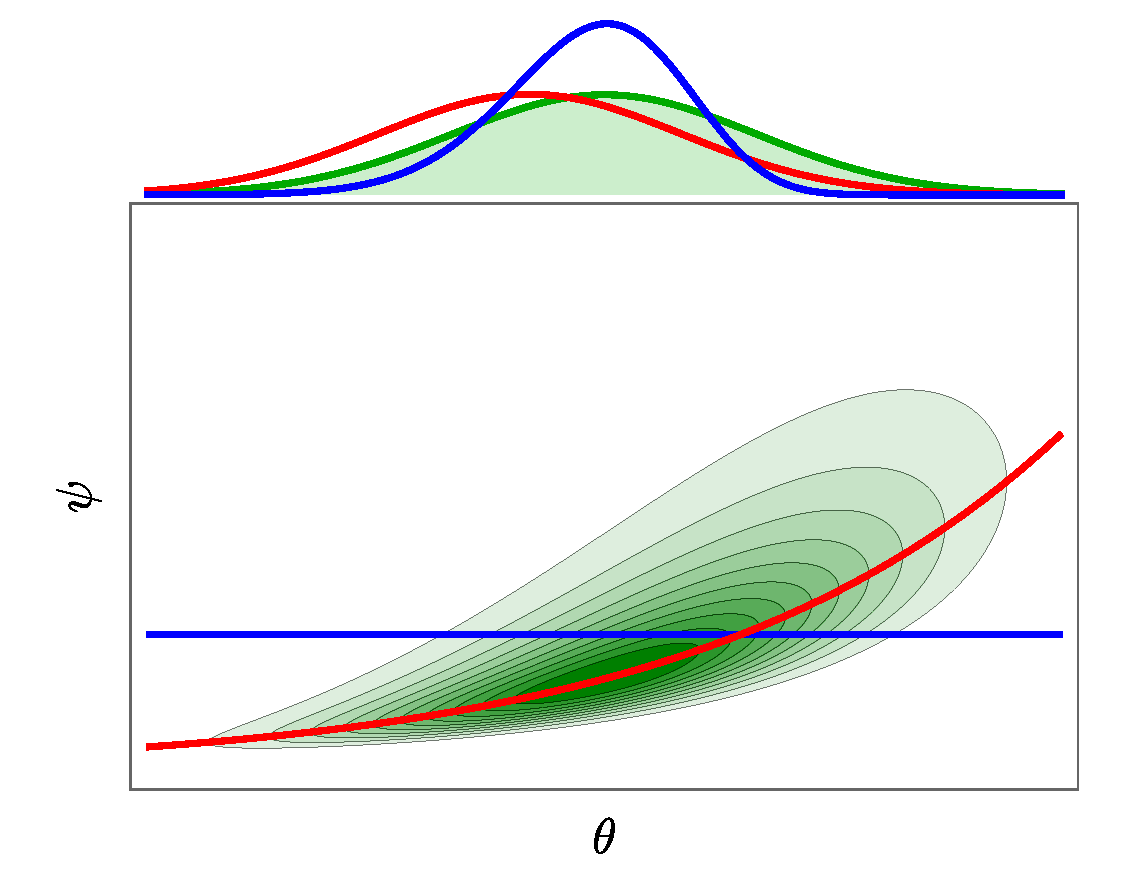
\includegraphics[width=10cm]{images/logo.pdf}}

\begin{document}

\maketitle

\tableofcontents
\listoflistings
\newpage

\section{Introduction}

This document is the technical documentation for the library \doclink{https://github.com/omarkahol/cmp.git}{CMP++}, a library primarily built for performing Bayesian calibration of computer models using several methods: 

\begin{enumerate}
    \item Full Bayes.
    \item Adaptive approaches (like CMP and FMP) .
    \item Sequential approaches (like KOH).
\end{enumerate}

The library also implements several Uncertainty Quantification (UQ) tools such as Gaussian Processes (GPs), Markov Chain Monte Carlo (MCMC) methods, Polynomial Chaos Expansions (PCE), Sobol sensitivity analysis and much more. The library is written entirely in C++ and currently provides no high level configuration file hence the pre-processing should be done using a C++ application.
The post-processing can be performed using any library or software capable of handling .csv input files. 

\smallskip
The library can be compiled as a static library or dynamic library and depends on the following libraries:

\begin{enumerate}
    \item \doclink{https://eigen.tuxfamily.org/index.php?title=Main_Page}{Eigen 3.4.0} for linear algebra.
    \item \doclink{https://nlopt.readthedocs.io/en/latest/}{NLopt 2.7.1} for gradient-free and gradient-based optimization.
    \item \doclink{https://www.csie.ntu.edu.tw/~cjlin/libsvm/}{LIBSVM} for support vector machines.
    \item \doclink{https://www.doxygen.nl}{Doxygen} to generate the documentation.
\end{enumerate}

These libraries should be installed in your system before proceeding. A detailed installation guide is provided in the next section. 
Furthermore, the test cases provided in the library use Matplotlib++ for plotting the results. Though this library is not required for the compilation of CMP++ it is strongly recommended to install it if you want to run the test cases. If you choose not to install it, you will have to modify the test cases accordingly and save the outputs as CVS files to be post-processed using another software.

\section{Installation}

This section is dedicated to the installation of the CMP++ library and its dependencies. Expert users can skip this section, install the dependencies themselves, compile CMP++ using the provided Makefile and link it to their target application either as a static or dynamic library. The following workflow is, however, strongly recommended.

\smallskip
First and foremost, make sure that you have a C++ compiler and cmake installed in your system. The latter can be checked by calling the following command in the terminal,

\begin{listing}[H]
\begin{minted}{bash}
make --version
\end{minted}
\end{listing}

The output should indicate the version installed. If this is the case, you can proceed to install the dependencies.

\subsection{Installing Eigen}
Eigen is a header only library so you just need to download the latest version from the \doclink{https://eigen.tuxfamily.org/index.php?title=Main_Page}{official website} and copy the folder into a known location. In this guide, I will assume that you have copied it into the folder HOME/opt/eigen-3.4.0 but you can choose whatever location you prefer. To use Eigen in your code, simply include the main header file

\begin{listing}[H]
\begin{minted}{c++}
#include <Eigen/Dense>
\end{minted}
\end{listing}

\subsection{Installing NLopt}
NLopt is compiled and linked as a dynamic library. This means that we will compile it as .dylib (in MacOs) file and we'll link it to our code during compilation. To install NLopt, you should download the latest version from the \doclink{https://nlopt.readthedocs.io/en/latest/}{official website}.

\smallskip
To install NLopt in HOME/opt copy the downloaded file in that folder and make sure that the name is something like nlopt-2.7.1 (otherwise simply rename the folder), access it via the terminal and type the following commands.

\begin{listing}[H]
\begin{minted}{bash}
mkdir build
cd build
cmake -DCMAKE_INSTALL_PREFIX=$HOME/opt/nlopt-2.7.1 ..
make
make install
\end{minted}
\end{listing}

This will compile the library into HOME/opt/nlopt-2.7.1 but you can change that by substituting HOME/opt in line 3 with whatever folder you desire. If the installation was successful, you should see that, in the nlopt folder you have an include folder which contains some \textbf{header files} and a lib folder which should contain (in MacOs) a \textbf{libnlopt.dylib} file. These two folders and files are the only one required so the rest can be safely removed. 

\smallskip
Now that we have compiled the library another operation must be performed. It is indeed necessary to append the lib folder path to the system path so that the executable knows where to look for the library during runtime. In MacOs, it is sufficient to add the following line to the .zshrc file in the home folder and restart the terminal 

\begin{listing}[H]
\begin{minted}{bash}
export DYLD_LIBRARY_PATH=${DYLD_LIBRARY_PATH}:$HOME/opt/nlopt-2.7.1/lib
\end{minted}
\end{listing}

If this is not properly done, your code will compile and link properly otherwise you will see an \textit{unresolved external symbol} error message at runtime.

\subsection{Installing LIBSVM}
LIBSVM is another library which is compiled and linked as a dynamic library. To install it, you should download the latest version from the \doclink{https://www.csie.ntu.edu.tw/~cjlin/libsvm/}{official website}. After downloading, compilation and linking is performed in a similar way as for NLopt.

\subsection{Installing CMP++}
In this subsection, I will show how to compile CMP++ as a static and dynamic library. First download the code the official GitHub repository and copy it into a known location. In this guide, I will assume that you have copied it into the folder HOME/opt/CMP++ but you can choose whatever location you prefer. To proceed, open the makefile in the base folder and modify the following lines according to your configuration,

\begin{listing}[H]
\begin{minted}{makefile}
# Define the C++ compiler to use
CXX = g++-15

# Define any compile-time flags
CXXFLAGS := -std=c++20 -O3 -fopenmp -mmacosx-version-min=14.0 -DNDEBUG
DEBUG_CXXFLAGS := -std=c++20 -g -O0 -fopenmp -mmacosx-version-min=14.0

# Define external includes
EIGEN = $(HOME)/opt/eigen-3.4.0/
NLOPTINC = $(HOME)/opt/nlopt-2.7.1/include
SELF = ./include
USR = /opt/homebrew/include
OMPINC = $(HOME)/opt/openmp/include
SVMINC = $(HOME)/opt/libsvm

# Define external libs
NLOPTLIB = $(HOME)/opt/nlopt-2.7.1/lib
OMPLIB = $(HOME)/opt/openmp/lib
SVMLIB = $(HOME)/opt/libsvm

\end{minted}
\end{listing}

The first variable should be modified to reflect the C++ compiler installed in your system. The second one contains the compilation flags which can be modified according to your needs. Right now CMP can be compiled both with debug flags and without, that's why you see two different CXXFLAGS variables. The next lines contain the path of the header and lib folders of the dependencies we installed in the previous sections. Make sure to modify them according to your configuration.

\smallskip
Finally, to compile CMP++ as a static library, simply access the CMP++ folder via the terminal and type \textit{make release} to compile it without debug flags, \textit{make debug} or \textit{make} to compile both versions.

\smallskip
If the compilation was successful, the lib folder should contain two files \textbf{libcmp.a} and \textbf{libcmp.dylib} which are the static and dynamic library respectively. If the debug version was compiled, the lib folder should also contain \textbf{libcmp\_debug.a} and \textbf{libcmp\_debug.dylib}.

\smallskip
This step should also generate the Doxygen documentation for the code in a folder called docs. To link against CMP++ in your code you should include the header files and link against the library. This can be done by adding the following lines to a makefile
\begin{listing}[H]
\begin{minted}{makefile}
# Define CMP++ includes
CMPINC = $(HOME)/opt/CMP++/include
CMPLIB = $(HOME)/opt/CMP++/lib
# Linking against CMP++ static library
LDFLAGS = -lcmp
\end{minted}
\end{listing}

\smallskip
Make sure to replace HOME/opt/CMP++ with the path where you have copied CMP++. See the provided test cases for more details.

\section{Test-cases and Verification}

This section presents the validation and verification of the CMP++ library using the provided test suite. For each test, we describe the underlying Uncertainty Quantification (UQ) and statistical learning methodology, present the rigorous mathematical formulation, detail the C++ implementation, and analyze the generated plots.

\subsection{Probability Distributions \& Sliced-Wasserstein Metrics}
This test case, implemented in \textbf{distribution.cpp}, validates the multivariate probability distribution module and Sliced-Wasserstein distance calculations. 

\subsubsection{Mathematical Formulation}
To draw samples from a Multivariate Normal Distribution $\mathcal{N}(\boldsymbol{\mu}, \boldsymbol{\Sigma})$, CMP++ performs an $\mathbf{L}\mathbf{D}\mathbf{L}^T$ decomposition (or Cholesky $\mathbf{L}\mathbf{L}^T$) of the covariance matrix:
\begin{equation}
    \boldsymbol{\Sigma} = \mathbf{L} \mathbf{D} \mathbf{L}^T \;,
\end{equation}
where $\mathbf{L}$ is a lower unit triangular matrix and $\mathbf{D}$ is a diagonal matrix. A sample is then drawn by generating $\mathbf{z} \sim \mathcal{N}(\mathbf{0}, \mathbf{I})$ and computing:
\begin{equation}
    \mathbf{x} = \boldsymbol{\mu} + \mathbf{L} \mathbf{D}^{1/2} \mathbf{z} \;.
\end{equation}

To verify that the generated empirical distribution converges to the target distribution, we compute the Sliced-Wasserstein distance. The $p$-Wasserstein distance between two probability measures $\mu$ and $\nu$ in $\mathbb{R}^d$ is defined via the optimal transport problem:
\begin{equation}
    W_p(\mu, \nu) = \left( \inf_{\gamma \in \Pi(\mu, \nu)} \int_{\mathbb{R}^d \times \mathbb{R}^d} \|\mathbf{x} - \mathbf{y}\|^p \, \mathrm{d}\gamma(\mathbf{x}, \mathbf{y}) \right)^{1/p} \;.
\end{equation}
Because optimal transport is computationally expensive in high dimensions, we project the high-dimensional distributions onto 1D lines. The Sliced-Wasserstein distance $SW_p$ is defined by integrating the 1D Wasserstein distances over the unit hypersphere $S^{d-1}$:
\begin{equation}
    SW_p(\mu, \nu) = \left( \frac{1}{|S^{d-1}|} \int_{S^{d-1}} W_p^p(\theta_\# \mu, \theta_\# \nu) \, \mathrm{d}\theta \right)^{1/p} \;,
\end{equation}
where $\theta_\# \mu$ denotes the push-forward of $\mu$ under the projection operator $\theta(\mathbf{x}) = \langle \mathbf{x}, \boldsymbol{\theta} \rangle$. Empirically, for a set of $L$ random projection angles $\{\boldsymbol{\theta}_l\}_{l=1}^L$, the distance is approximated as:
\begin{equation}
    SW_p^p(\mu, \nu) \approx \frac{1}{L} \sum_{l=1}^L W_p^p\left( \{\langle \mathbf{x}_i, \boldsymbol{\theta}_l \rangle\}_{i=1}^N, \{\langle \mathbf{y}_j, \boldsymbol{\theta}_l \rangle\}_{j=1}^N \right) \;,
\end{equation}
where the 1D Wasserstein distance between the projected sorted samples is computed simply as $\frac{1}{N} \sum_{i=1}^N |x_{(i)} - y_{(i)}|^p$.

\subsubsection{C++ Implementation \& Verification}
In this test, a 2D Multivariate Normal distribution is defined with:
\begin{equation}
    \boldsymbol{\mu} = \begin{bmatrix} 0.0 \\ 0.0 \end{bmatrix}, \quad \boldsymbol{\Sigma} = \begin{bmatrix} 1.0 & 0.8 \\ 0.8 & 1.0 \end{bmatrix} \;.
\end{equation}
We draw 10,000 samples and plot them to verify correlation.

\begin{figure}[H]
    \centering
    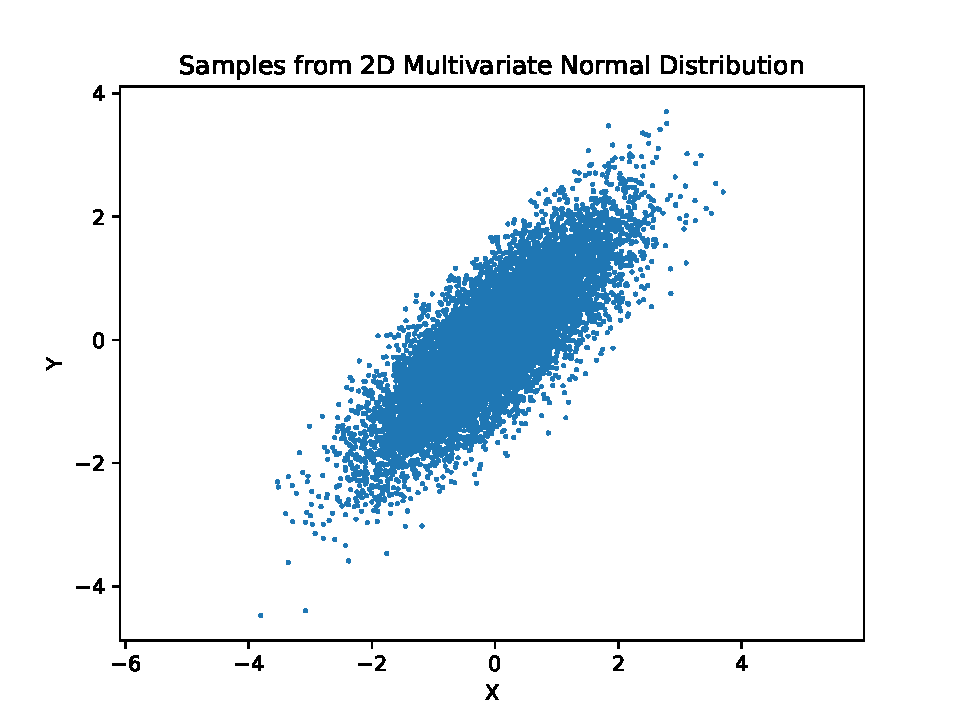
\includegraphics[width=0.65\textwidth]{images/distribution_mvn.pdf}
    \caption{Samples drawn from the 2D Multivariate Normal distribution, showcasing the strong positive correlation ($\rho = 0.8$).}
    \label{fig:mvn_samples}
\end{figure}

The computed Sliced-Wasserstein distance ($p=2, 100\text{ slices}$) between two independent batches of $5,000$ samples is approximately $1.3 \times 10^{-4}$, confirming that the sampler generates statistically indistinguishable realizations from the target density.

\subsection{Markov Chain Monte Carlo (MCMC) Diagnostics}
The test case \textbf{mcmc.cpp} samples a highly bimodal posterior distribution:
\begin{equation}
    \log p(x) \propto -10 \left(x^2 - 1\right)^2 \;,
\end{equation}
which has modes at $x = \pm 1$.

\subsubsection{Mathematical Formulation}
At each step of the Metropolis-Hastings (MH) algorithm, a candidate $y$ is proposed from $q(y|x)$ and accepted with probability:
\begin{equation}
    \alpha(x, y) = \min\left(1, \frac{p(y) q(x|y)}{p(x) q(y|x)}\right) \;.
\end{equation}
In Delayed Rejection (DR), if a proposal $y_1$ is rejected, a second-stage proposal $y_2$ is generated from $q_2(y_2|x, y_1)$. The second-stage acceptance probability is:
\begin{equation}
    \alpha_2(x, y_1, y_2) = \min\left(1, \frac{p(y_2) q_1(y_1|y_2) q_2(x|y_1, y_2) [1 - \alpha_1(y_2, y_1)]}{p(x) q_1(y_1|x) q_2(y_2|x, y_1) [1 - \alpha_1(x, y_1)]}\right) \;.
\end{equation}
In Adaptive Metropolis (AM), the proposal covariance $\boldsymbol{\Sigma}_t$ is updated based on the history of the chain:
\begin{equation}
    \boldsymbol{\Sigma}_t = s_d \operatorname{Cov}(x_0, \dots, x_{t-1}) + s_d \varepsilon \mathbf{I}_d \;,
\end{equation}
where $s_d = 2.38^2 / d$ is the optimal scaling factor and $\varepsilon$ is a small nugget for stability.

The autocorrelation function of a chain $\{x_t\}_{t=1}^N$ at lag $k$ is computed using FFT for speed:
\begin{equation}
    \rho(k) = \frac{\mathbb{E}[(x_t - \mu)(x_{t+k} - \mu)]}{\sigma^2} \;.
\end{equation}
The Effective Sample Size (ESS) is defined as:
\begin{equation}
    \text{ESS} = \frac{N}{1 + 2 \sum_{k=1}^\infty \rho(k)} \;.
\end{equation}

\subsubsection{C++ Implementation \& Verification}
We run the DRAM sampler, discard the first $10,000$ samples as burn-in, draw $1,000,000$ samples, and thin the chain by a factor of 10.

\begin{figure}[H]
    \centering
    \begin{minipage}{0.48\textwidth}
        \centering
        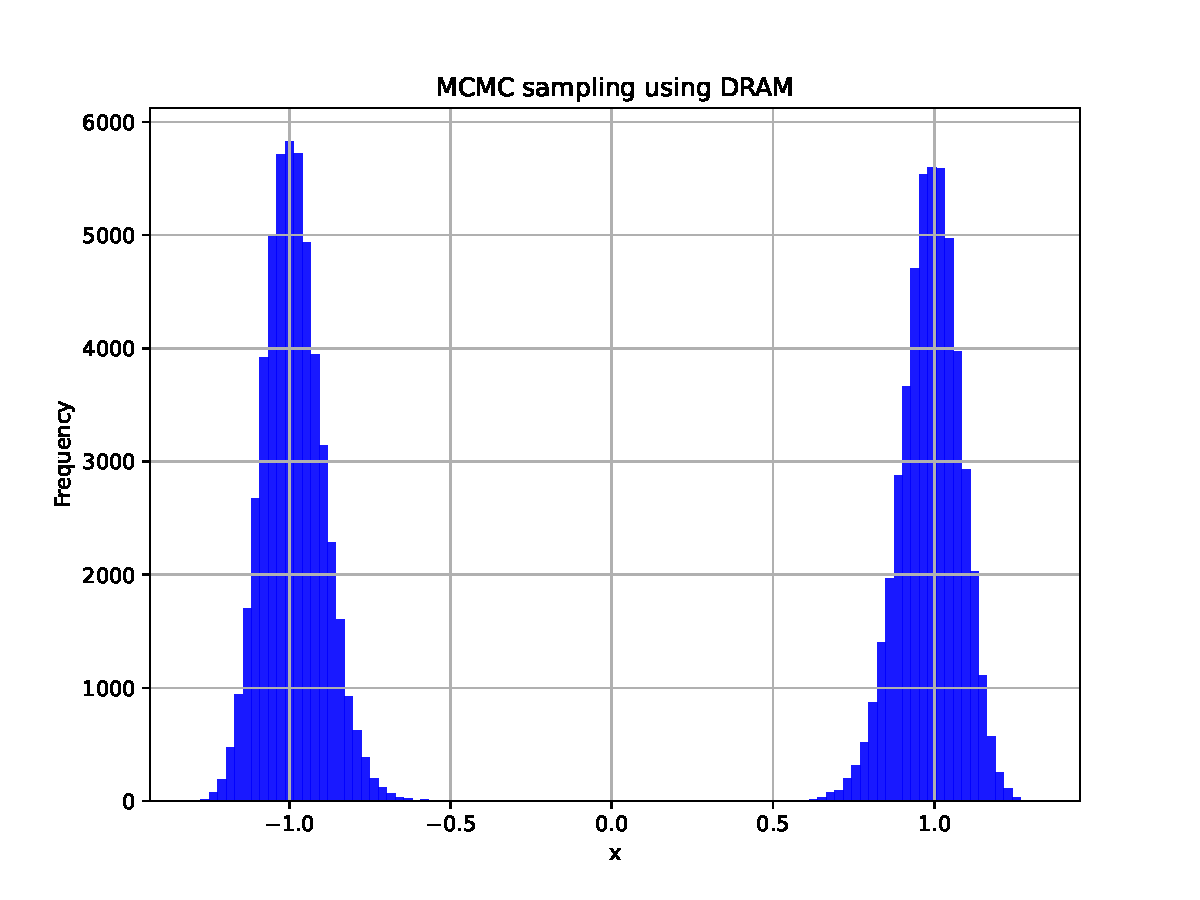
\includegraphics[width=\textwidth]{images/mcmc.pdf}
        \caption{Empirical histogram of MCMC samples showing successful capturing of the bimodal distribution.}
        \label{fig:mcmc_hist}
    \end{minipage}
    \hfill
    \begin{minipage}{0.48\textwidth}
        \centering
        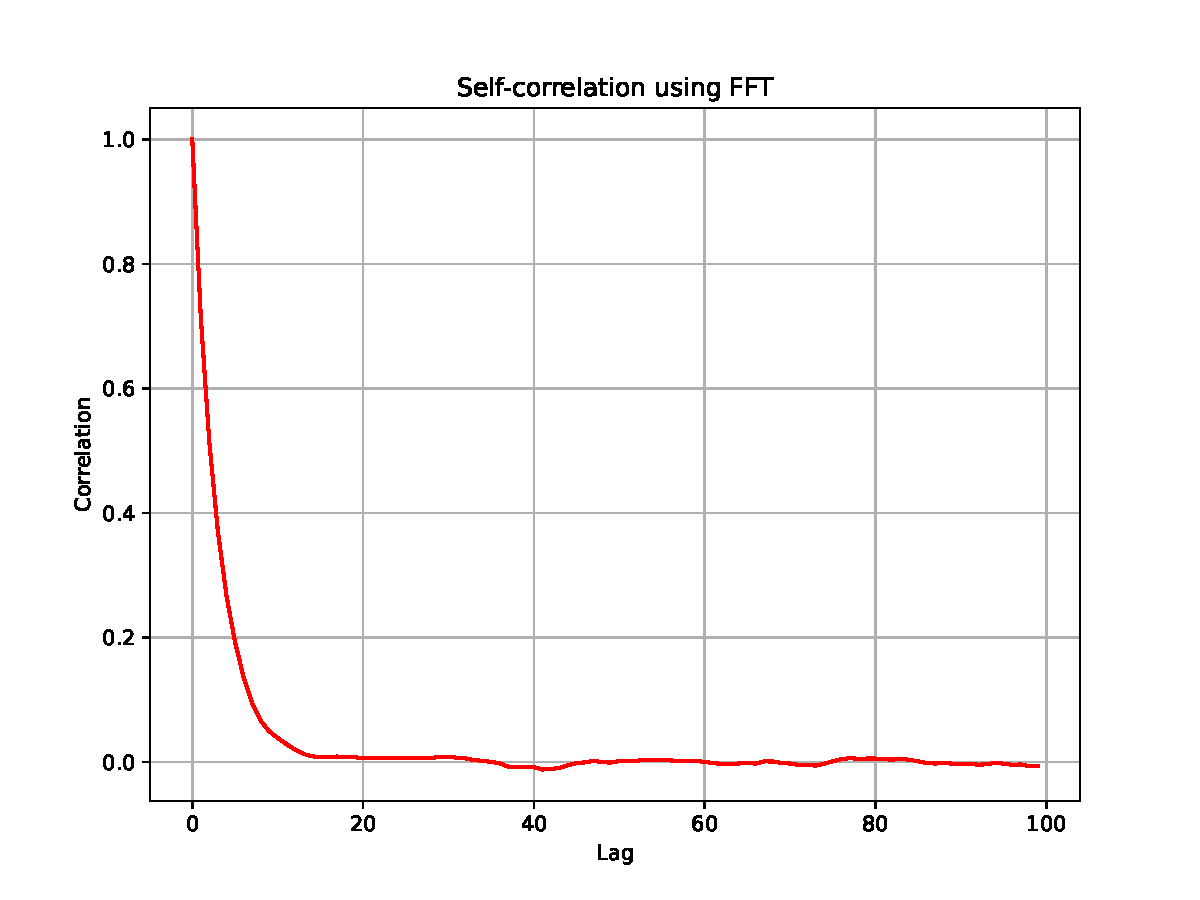
\includegraphics[width=\textwidth]{images/mcmc_autocorr.pdf}
        \caption{Autocorrelation function of the chain computed efficiently via FFT.}
        \label{fig:mcmc_autocorr}
    \end{minipage}
\end{figure}

The diagnostic output yields a self-correlation length of approximately $3.7$ steps and an ESS of over $15,500$, proving high sampling efficiency and low correlation between samples.

\subsection{Kernel Density Estimation (KDE)}
Implemented in \textbf{kde.cpp}, this test demonstrates non-parametric density estimation.

\subsubsection{Mathematical Formulation}
For a dataset $\{\mathbf{x}_i\}_{i=1}^N$ in $\mathbb{R}^d$, the Kernel Density Estimator is:
\begin{equation}
    \hat{f}_{\mathbf{H}}(\mathbf{x}) = \frac{1}{N} \sum_{i=1}^N K_{\mathbf{H}}(\mathbf{x} - \mathbf{x}_i) \;,
\end{equation}
where $K_{\mathbf{H}}(\mathbf{z}) = |\mathbf{H}|^{-1/2} K(\mathbf{H}^{-1/2} \mathbf{z})$, with $\mathbf{H}$ being the symmetric positive-definite bandwidth matrix.
The multivariate Gaussian kernel is:
\begin{equation}
    K(\mathbf{z}) = (2\pi)^{-d/2} \exp\left(-\frac{1}{2} \|\mathbf{z}\|^2 \right) \;.
\end{equation}
Silverman's rule of thumb selects a diagonal bandwidth matrix $\mathbf{H}_{jj} = h_j^2$ where:
\begin{equation}
    h_j = \left(\frac{4}{d+2}\right)^{\frac{1}{d+4}} N^{-\frac{1}{d+4}} \sigma_j \;,
\end{equation}
with $\sigma_j$ being the standard deviation of the $j$-th coordinate.
The bandwidth matrix is optimized by maximizing the Leave-One-Out Likelihood Cross-Validation (LOOCV) score:
\begin{equation}
    \text{LOOCV}(\mathbf{H}) = \sum_{i=1}^N \log \hat{f}_{\mathbf{H},-i}(\mathbf{x}_i) \;,
\end{equation}
where $\hat{f}_{\mathbf{H},-i}$ is the KDE constructed omitting the $i$-th observation.

\subsubsection{C++ Implementation \& Verification}
We generate $1,000$ samples from a Gaussian Mixture Model (GMM) with weights $0.3$ and $0.7$:
\begin{equation}
    p(\mathbf{x}) = 0.3 \cdot \mathcal{N}\left(\mathbf{x}; \boldsymbol{\mu}_1, \boldsymbol{\Sigma}_1\right) + 0.7 \cdot \mathcal{N}\left(\mathbf{x}; \boldsymbol{\mu}_2, \boldsymbol{\Sigma}_2\right) \;,
\end{equation}
where $\boldsymbol{\mu}_1 = [-0.5, 0.5]^T$ and $\boldsymbol{\mu}_2 = [0.5, -0.5]^T$.

\begin{figure}[H]
    \centering
    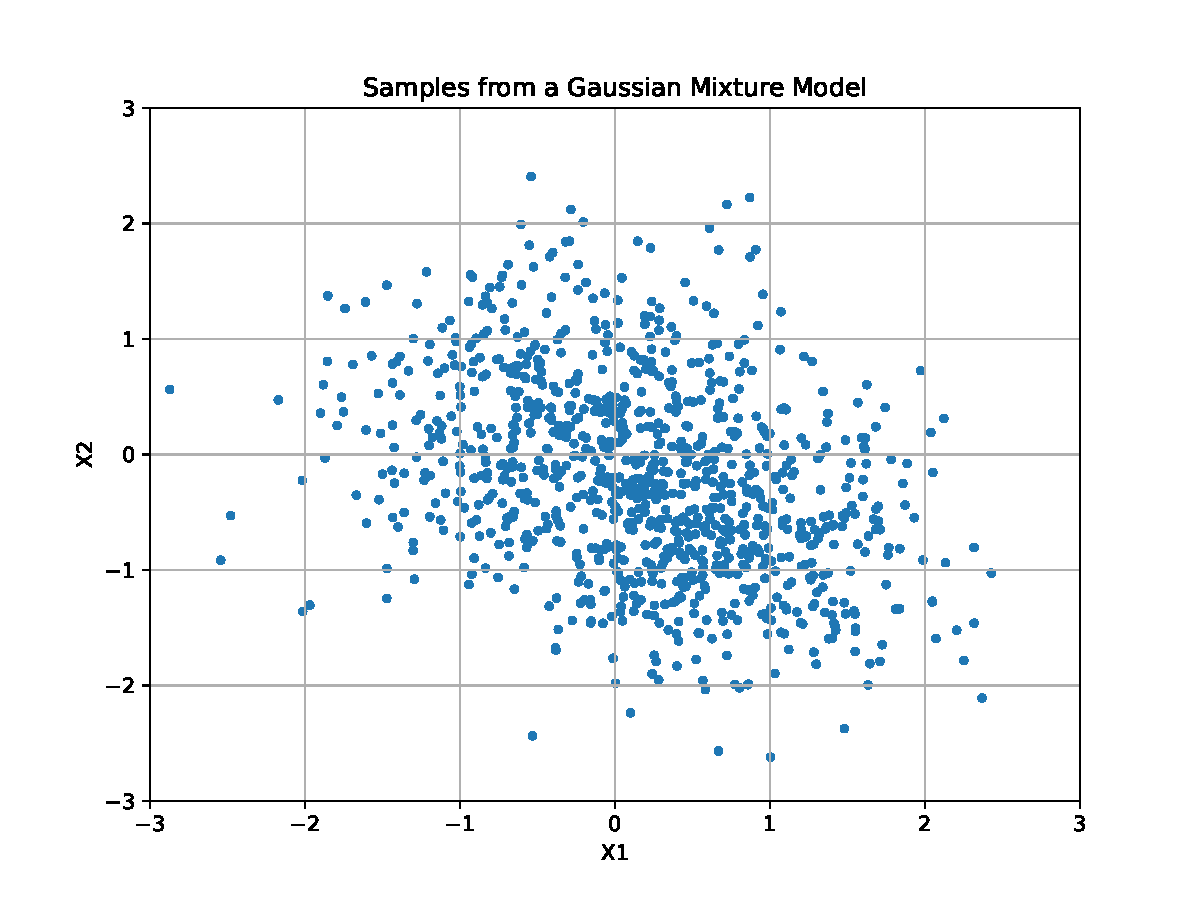
\includegraphics[width=0.6\textwidth]{images/mixture.pdf}
    \caption{Scatter plot of GMM samples.}
    \label{fig:mixture_samples}
\end{figure}

The true density at origin is $0.202$. The Silverman KDE yields $0.156$ with bandwidth:
\begin{equation}
    \mathbf{H} = \begin{bmatrix} 0.243 & 0.0 \\ 0.0 & 0.241 \end{bmatrix} \;.
\end{equation}
Maximizing the LOOCV score refines the bandwidth to:
\begin{equation}
    \mathbf{H}_{\text{opt}} = \begin{bmatrix} 0.065 & -0.008 \\ -0.008 & 0.076 \end{bmatrix} \;,
\end{equation}
which brings the estimated density at origin to $0.196$, validating the optimization.

\subsection{Supervised Classification: KDE, SVM, and Multi-class Decision Boundaries}
The file \textbf{classifier.cpp} compares KDE and Support Vector Machine (SVM) binary classifiers on the synthetic 2D moons dataset. 

\subsubsection{Mathematical Formulation}
The Support Vector Machine (SVM) binary classifier constructs a decision boundary by finding the hyperplane that maximizes the margin. In kernelized dual form, we solve:
\begin{equation}
    \max_{\boldsymbol{\alpha}} \sum_{i=1}^N \alpha_i - \frac{1}{2} \sum_{i=1}^N \sum_{j=1}^N \alpha_i \alpha_j y_i y_j K(\mathbf{x}_i, \mathbf{x}_j) \;,
\end{equation}
subject to $0 \le \alpha_i \le C$ and $\sum_{i=1}^N \alpha_i y_i = 0$.
The Radial Basis Function (RBF) kernel is defined as:
\begin{equation}
    K(\mathbf{x}, \mathbf{x}') = \exp\left( - \gamma \|\mathbf{x} - \mathbf{x}'\|^2 \right) \;.
\end{equation}
Hyperparameter tuning of $C$ and $\gamma$ is performed using a span-bound estimate to minimize the leave-one-out error.

\subsubsection{C++ Implementation \& Verification}
We compare the classification decision boundaries generated by the optimized KDE and SVM.

\begin{figure}[H]
    \centering
    \begin{minipage}{0.32\textwidth}
        \centering
        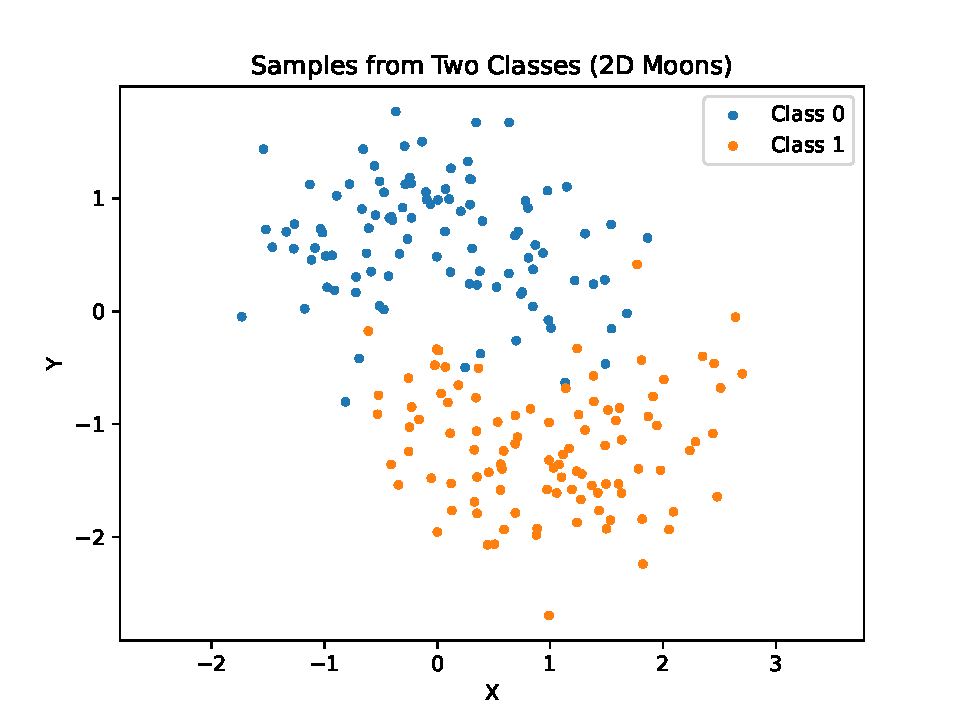
\includegraphics[width=\textwidth]{images/moons.pdf}
        \caption{Raw moons dataset.}
        \label{fig:moons_raw}
    \end{minipage}
    \hfill
    \begin{minipage}{0.32\textwidth}
        \centering
        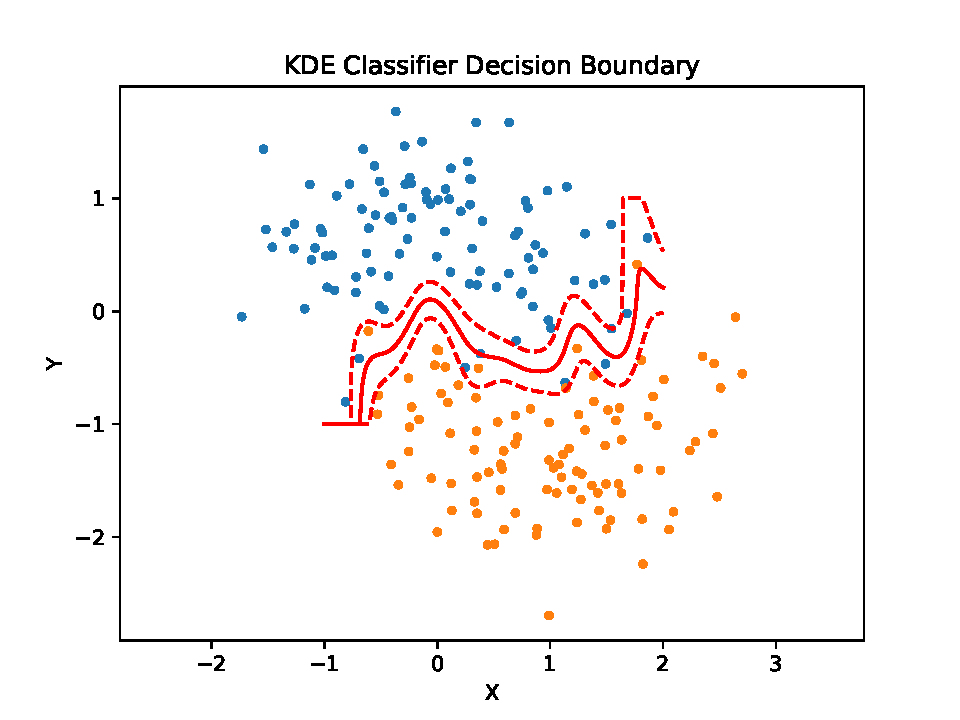
\includegraphics[width=\textwidth]{images/kde.pdf}
        \caption{KDE decision boundary.}
        \label{fig:moons_kde}
    \end{minipage}
    \hfill
    \begin{minipage}{0.32\textwidth}
        \centering
        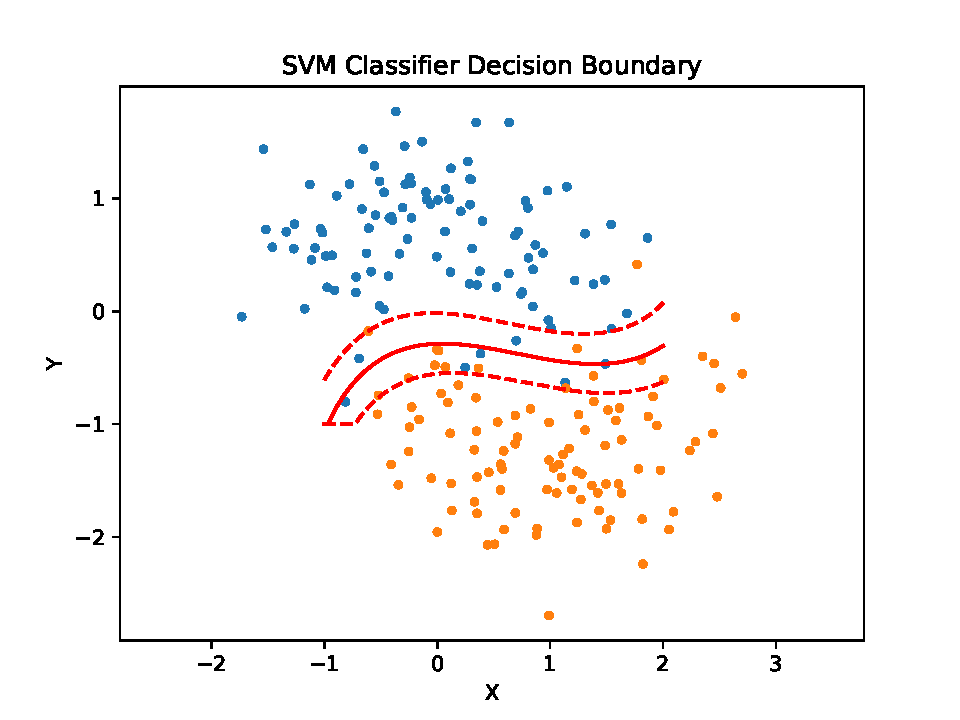
\includegraphics[width=\textwidth]{images/svm.pdf}
        \caption{SVM decision boundary.}
        \label{fig:moons_svm}
    \end{minipage}
\end{figure}

Additionally, \textbf{svm.cpp} performs multi-class SVM classification on a complex 10-class dataset, finding optimized RBF parameters ($\gamma = 0.14$, $C = 10.14$) and achieving a training accuracy of $98\%$.

\begin{figure}[H]
    \centering
    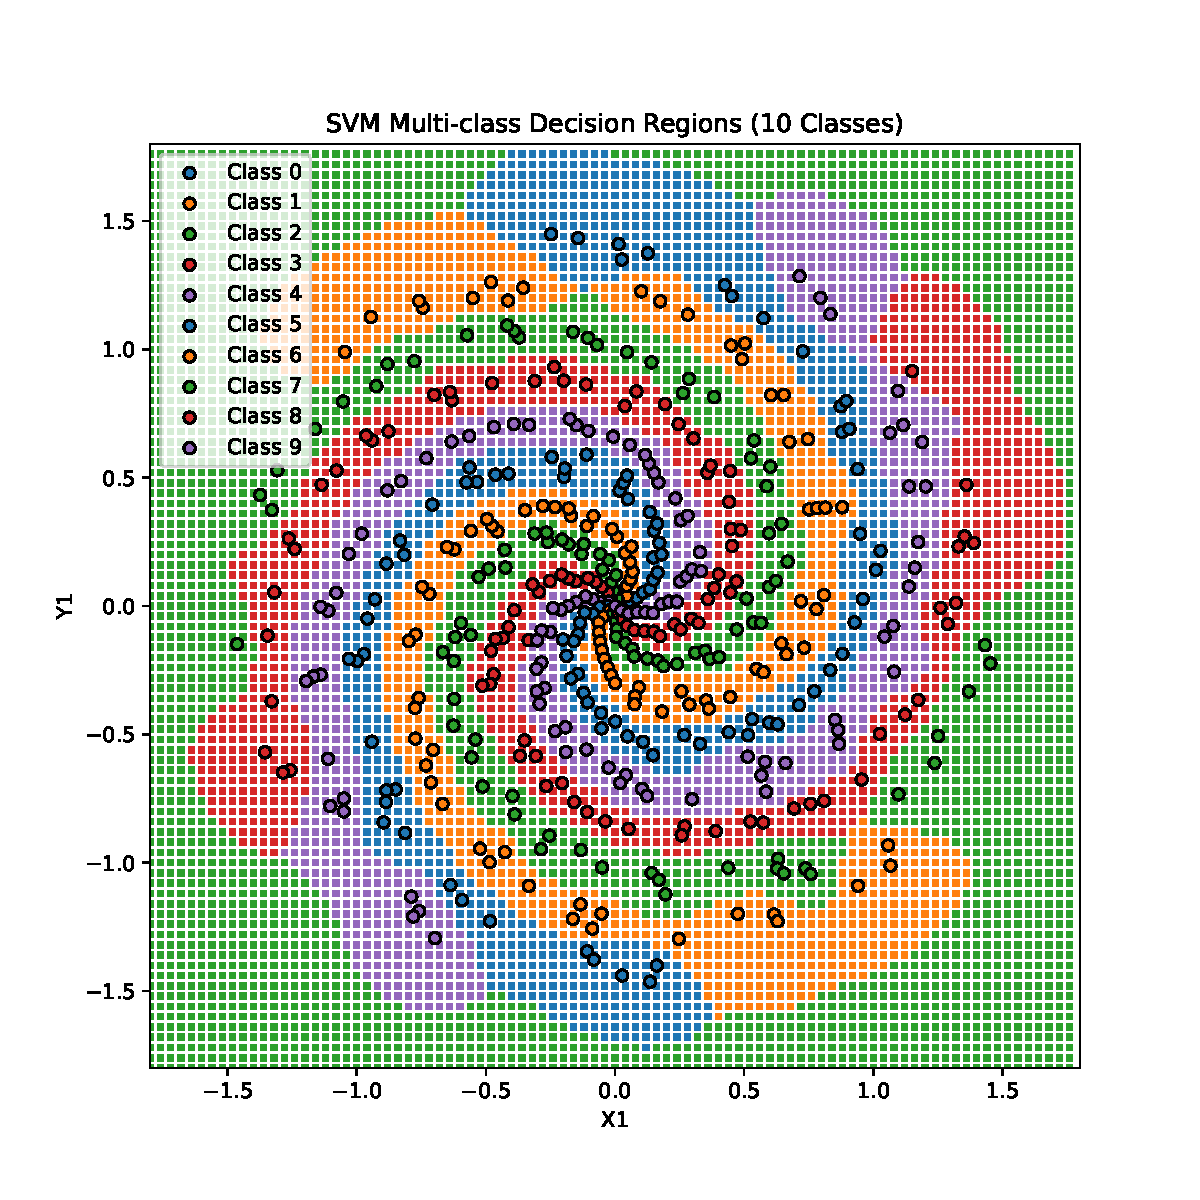
\includegraphics[width=0.6\textwidth]{images/svm_multiclass.pdf}
    \caption{Decision regions for the 10-class SVM classifier.}
    \label{fig:svm_multiclass}
\end{figure}

\subsection{Gaussian Process (GP) Regression}
Implemented in \textbf{gp.cpp}, this test conditions a Gaussian Process model on noisy data generated from $y = \sin(2\pi x) + 1 + \varepsilon$.

\subsubsection{Mathematical Formulation}
A Gaussian Process is a collection of random variables, any finite number of which have a joint Gaussian distribution. It is completely defined by its mean function $m(\mathbf{x})$ and covariance function $k(\mathbf{x}, \mathbf{x}')$:
\begin{equation}
    f(\mathbf{x}) \sim \mathcal{GP}\left(m(\mathbf{x}), k(\mathbf{x}, \mathbf{x}')\right) \;.
\end{equation}
Given training observations $\mathbf{y}$ at inputs $\mathbf{X}$, the joint distribution of training outputs and prediction outputs $\mathbf{f}_*$ at test points $\mathbf{X}_*$ is:
\begin{equation}
    \begin{bmatrix} \mathbf{y} \\ \mathbf{f}_* \end{bmatrix} \sim \mathcal{N}\left( \begin{bmatrix} m(\mathbf{X}) \\ m(\mathbf{X}_*) \end{bmatrix}, \begin{bmatrix} \mathbf{K}(\mathbf{X}, \mathbf{X}) + \sigma_n^2 \mathbf{I} & \mathbf{K}(\mathbf{X}, \mathbf{X}_*) \\ \mathbf{K}(\mathbf{X}_*, \mathbf{X}) & \mathbf{K}(\mathbf{X}_*, \mathbf{X}_*) \end{bmatrix} \right) \;.
\end{equation}
Conditioning on $\mathbf{y}$ yields the posterior distribution $\mathbf{f}_* | \mathbf{X}, \mathbf{y}, \mathbf{X}_* \sim \mathcal{N}(\bar{\mathbf{f}}_*, \operatorname{cov}(\mathbf{f}_*))$:
\begin{equation}
    \bar{\mathbf{f}}_* = m(\mathbf{X}_*) + \mathbf{K}(\mathbf{X}_*, \mathbf{X}) \left[ \mathbf{K}(\mathbf{X}, \mathbf{X}) + \sigma_n^2 \mathbf{I} \right]^{-1} (\mathbf{y} - m(\mathbf{X})) \;,
\end{equation}
\begin{equation}
    \operatorname{cov}(\mathbf{f}_*) = \mathbf{K}(\mathbf{X}_*, \mathbf{X}_*) - \mathbf{K}(\mathbf{X}_*, \mathbf{X}) \left[ \mathbf{K}(\mathbf{X}, \mathbf{X}) + \sigma_n^2 \mathbf{I} \right]^{-1} \mathbf{K}(\mathbf{X}, \mathbf{X}_*) \;.
\end{equation}
We optimize the hyperparameters $\boldsymbol{\theta} = (\sigma_f, \ell, \sigma_n)$ of the Squared Exponential kernel by minimizing the Leave-One-Out (LOO) cross-validation Mean Squared Error:
\begin{equation}
    \text{MSE}_{\text{LOO}} = \frac{1}{N} \sum_{i=1}^N \left( y_i - \hat{\mu}_{-i}(x_i) \right)^2 \;,
\end{equation}
where $\hat{\mu}_{-i}(x_i)$ is the GP prediction at $x_i$ computed by omitting the $i$-th observation.

\subsubsection{C++ Implementation \& Verification}
We compare the prior GP, the conditioned posterior GP, and the optimized posterior GP.

\begin{figure}[H]
    \centering
    \begin{minipage}{0.32\textwidth}
        \centering
        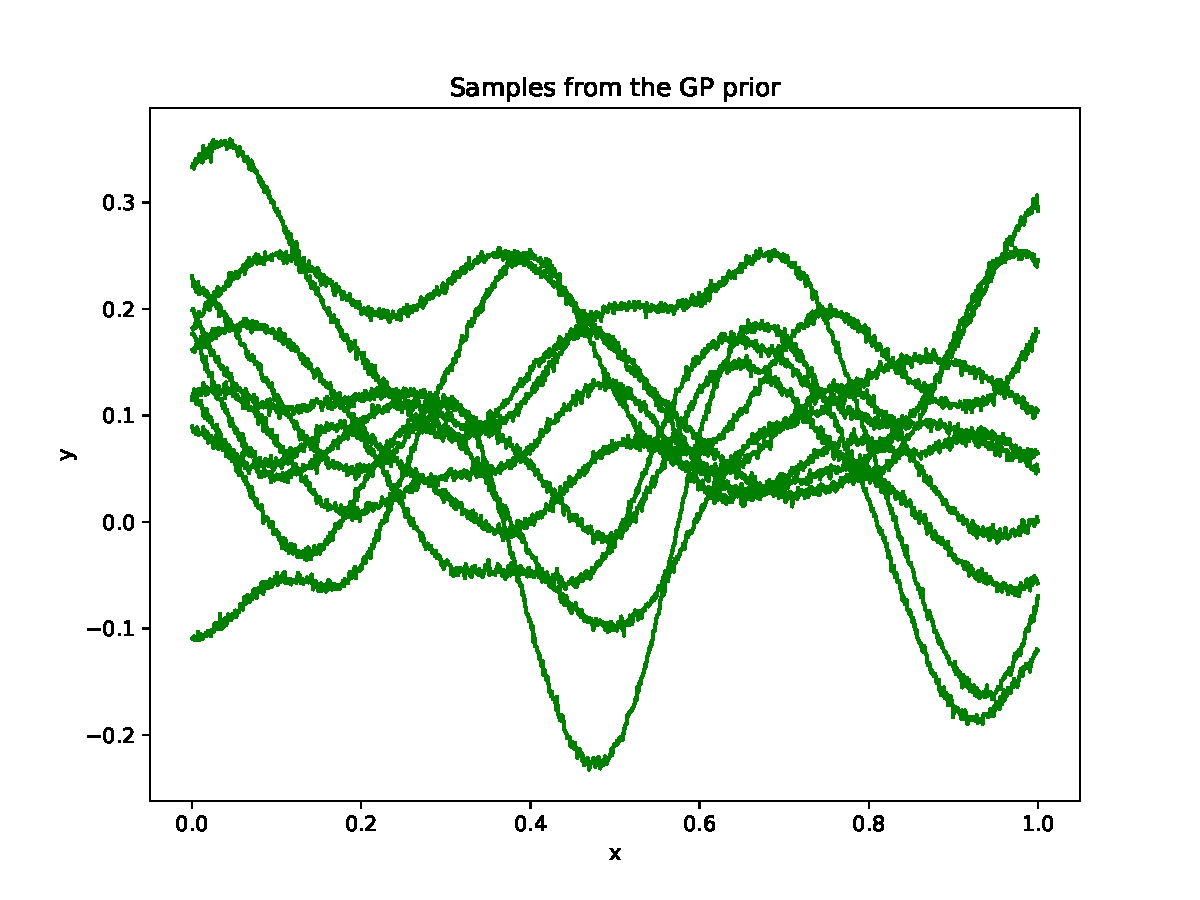
\includegraphics[width=\textwidth]{images/gp_prior.pdf}
        \caption{Samples from GP prior.}
        \label{fig:gp_prior}
    \end{minipage}
    \hfill
    \begin{minipage}{0.32\textwidth}
        \centering
        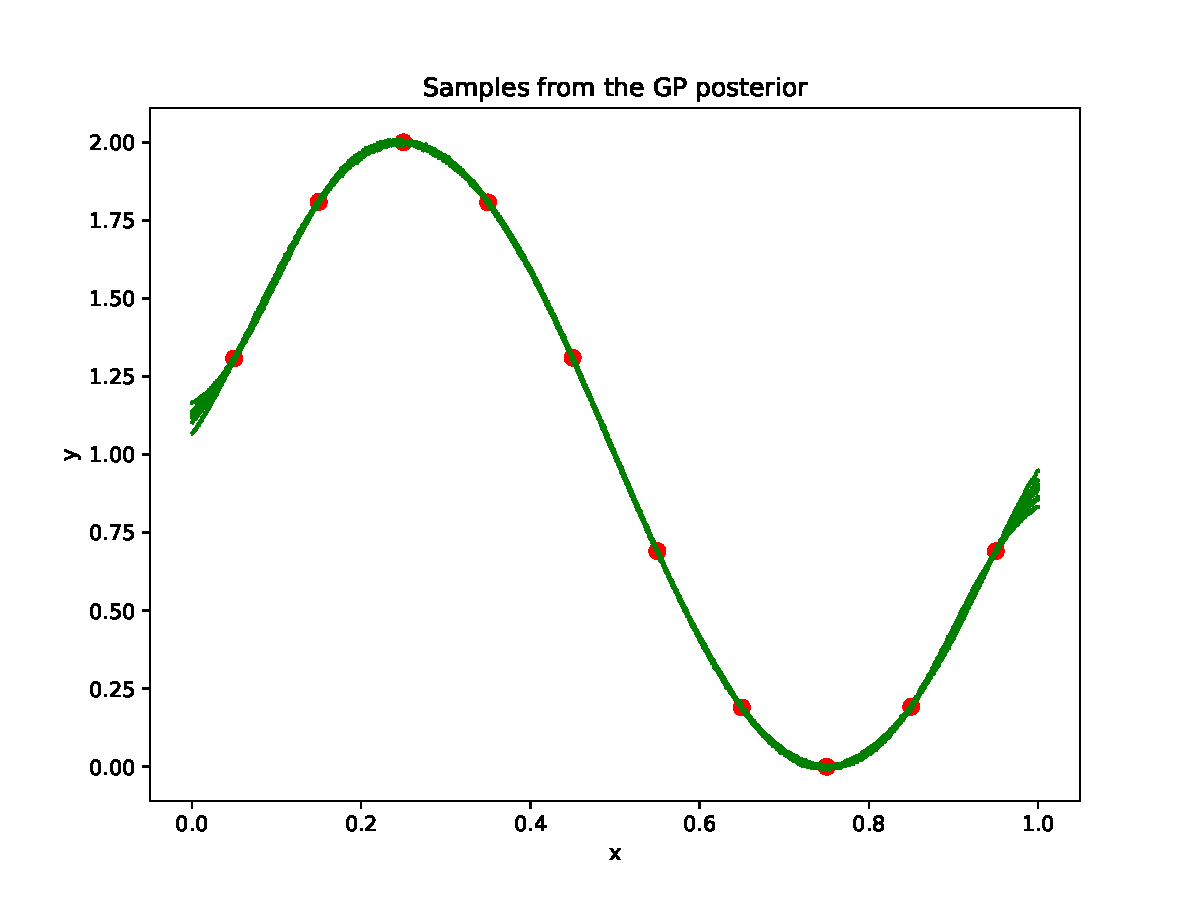
\includegraphics[width=\textwidth]{images/gp_posterior.pdf}
        \caption{Samples from posterior.}
        \label{fig:gp_posterior}
    \end{minipage}
    \hfill
    \begin{minipage}{0.32\textwidth}
        \centering
        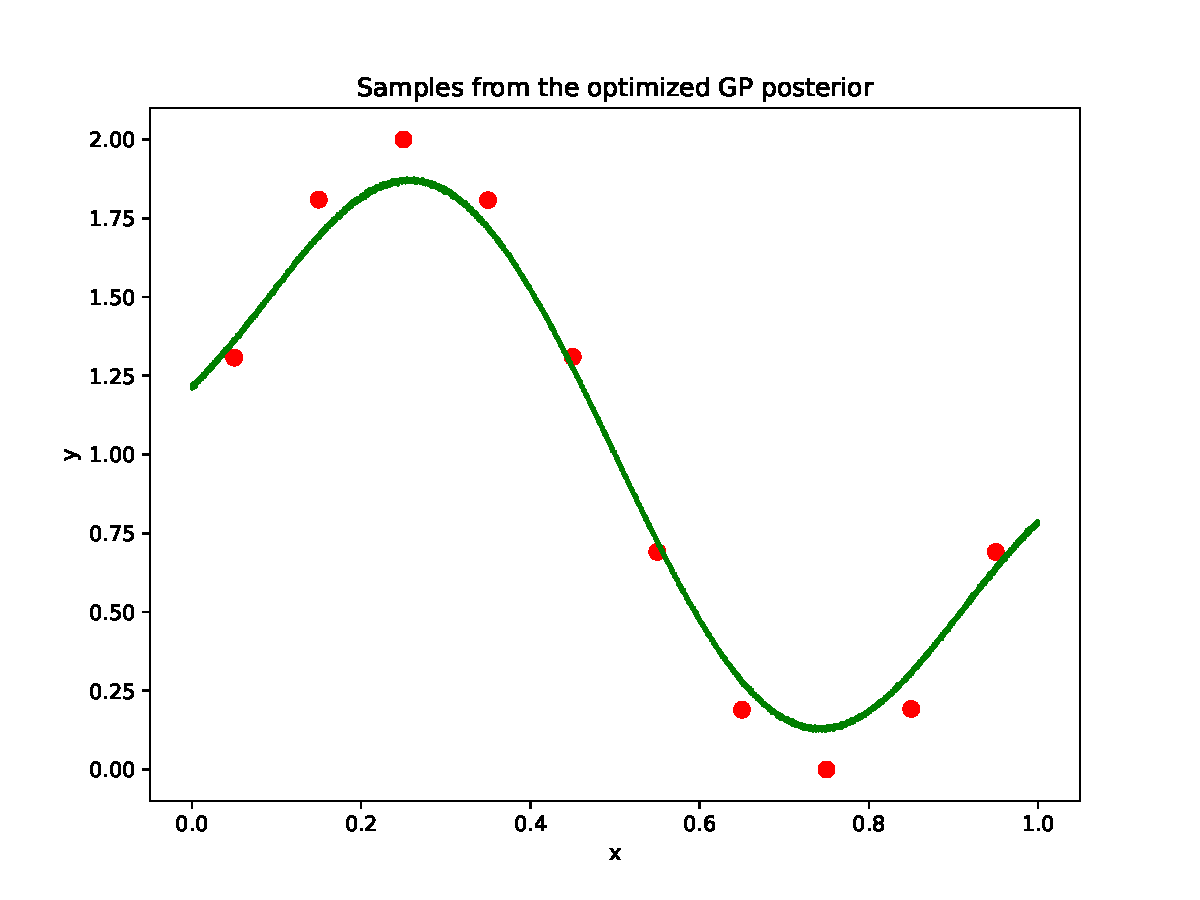
\includegraphics[width=\textwidth]{images/gp_posterior_opt.pdf}
        \caption{Samples from optimized posterior.}
        \label{fig:gp_posterior_opt}
    \end{minipage}
\end{figure}

The cross-validation MSE drops from $0.302$ (initial hyperparameters) to $0.040$ after optimization, demonstrating the importance of hyperparameter optimization.

\subsection{Multi-Output GP with Dimensionality Reduction}
The test case \textbf{multi\_gp.cpp} fits a multi-output GP using Principal Component Analysis (PCA) to project a highly correlated 3D output vector into a 2D latent space.

\subsubsection{Mathematical Formulation}
For a multi-output training matrix $\mathbf{Y} \in \mathbb{R}^{N \times D}$ (where $D=3$ is high-dimensional), we compute the singular value decomposition (SVD) of the centered matrix to obtain the projection matrix $\mathbf{W} \in \mathbb{R}^{D \times r}$ corresponding to the top $r=2$ principal components:
\begin{equation}
    \mathbf{Z} = (\mathbf{Y} - \mathbf{1}\boldsymbol{\mu}^T) \mathbf{W} \;,
\end{equation}
where $\mathbf{Z} \in \mathbb{R}^{N \times r}$ is the matrix of low-dimensional latent coordinates. We fit $r$ independent Gaussian Processes to each column of $\mathbf{Z}$. Predictions at test inputs are projected back to the physical space:
\begin{equation}
    \hat{\mathbf{Y}}_* = \hat{\mathbf{Z}}_* \mathbf{W}^T + \mathbf{1}\boldsymbol{\mu}^T \;,
\end{equation}
with the prediction covariance similarly mapped.

\subsubsection{C++ Implementation \& Verification}
We fit the multi-output GP and verify the reconstructions against observations.

\begin{figure}[H]
    \centering
    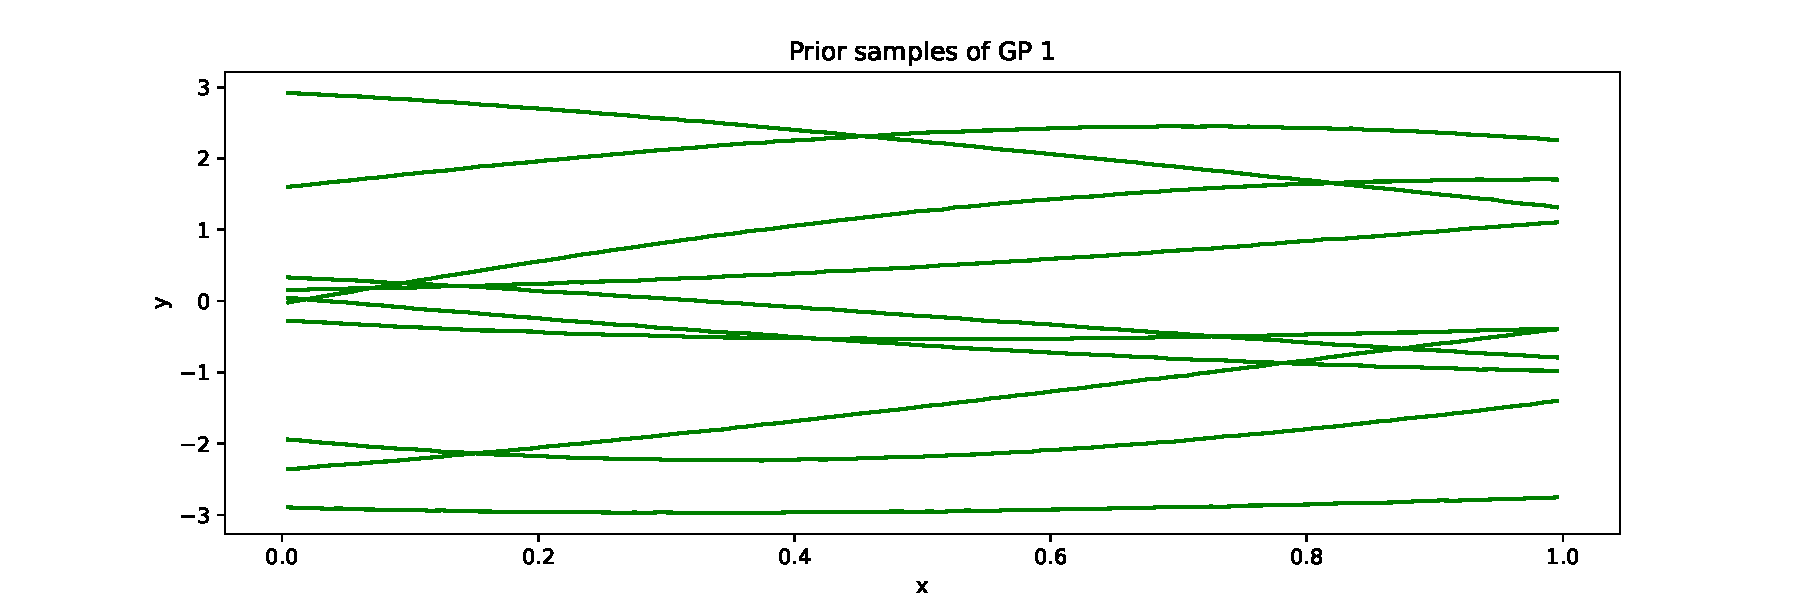
\includegraphics[width=0.45\textwidth]{images/multi_gp_prior.pdf}
    \caption{GP prior samples for the latent dimensions.}
    \label{fig:multi_gp_prior}
\end{figure}

\begin{figure}[H]
    \centering
    \begin{minipage}{0.32\textwidth}
        \centering
        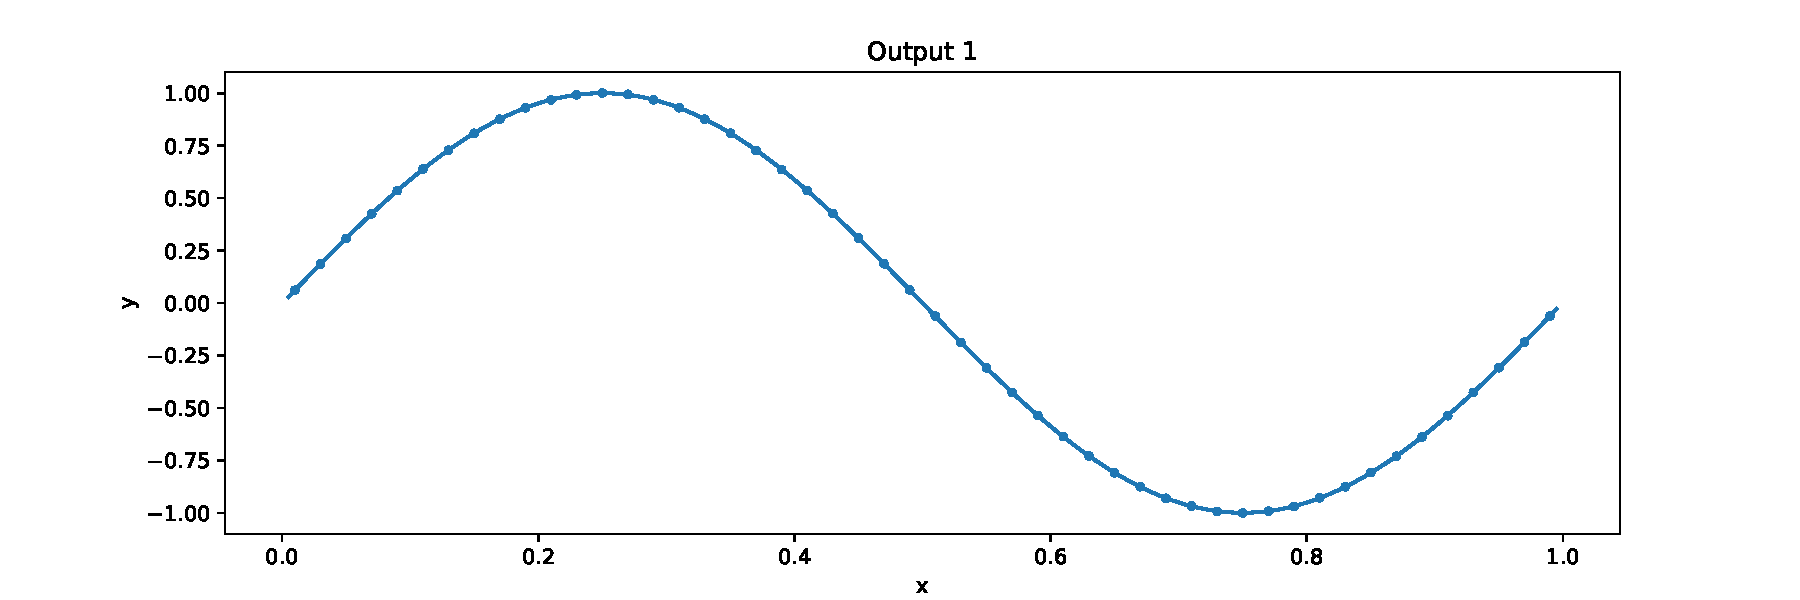
\includegraphics[width=\textwidth]{images/multi_gp_output_1.pdf}
        \caption{Output 1 regression.}
    \end{minipage}
    \hfill
    \begin{minipage}{0.32\textwidth}
        \centering
        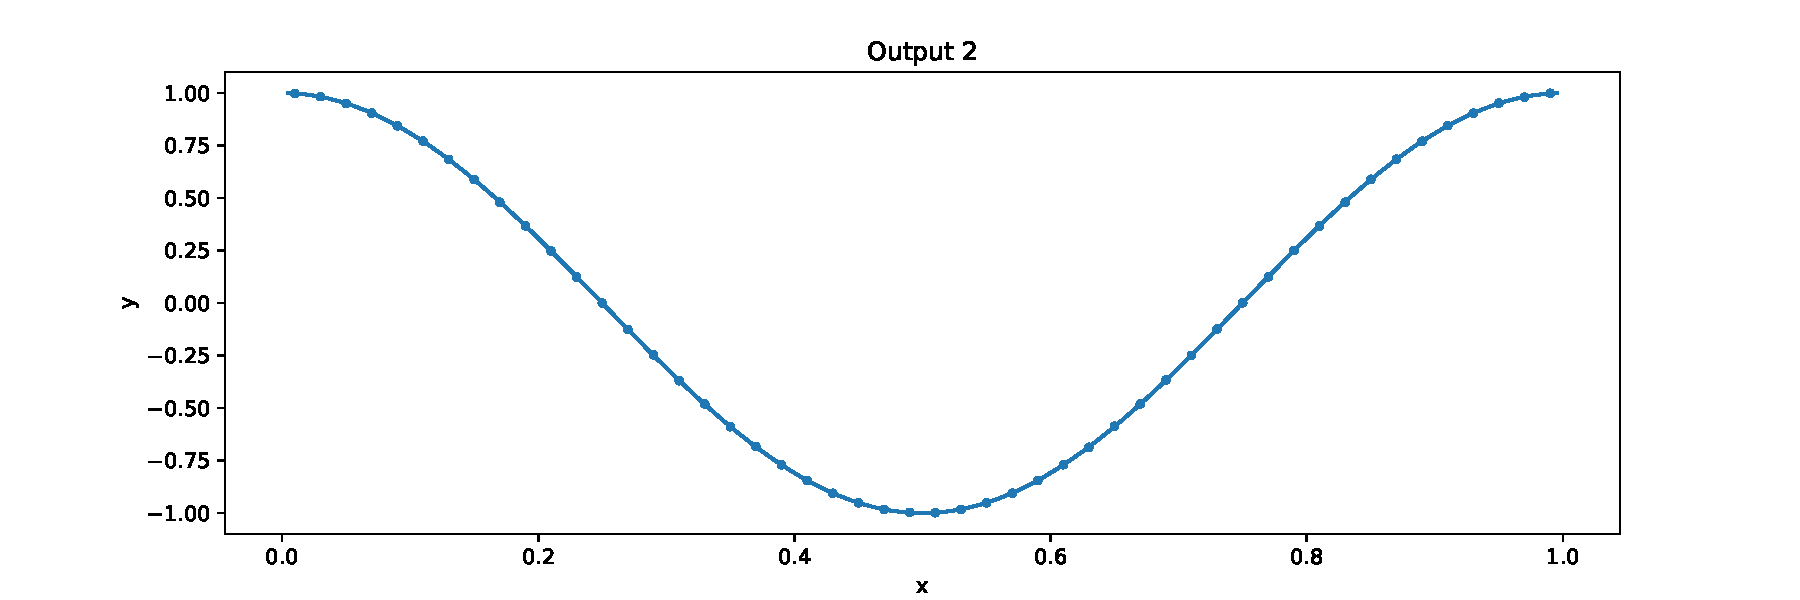
\includegraphics[width=\textwidth]{images/multi_gp_output_2.pdf}
        \caption{Output 2 regression.}
    \end{minipage}
    \hfill
    \begin{minipage}{0.32\textwidth}
        \centering
        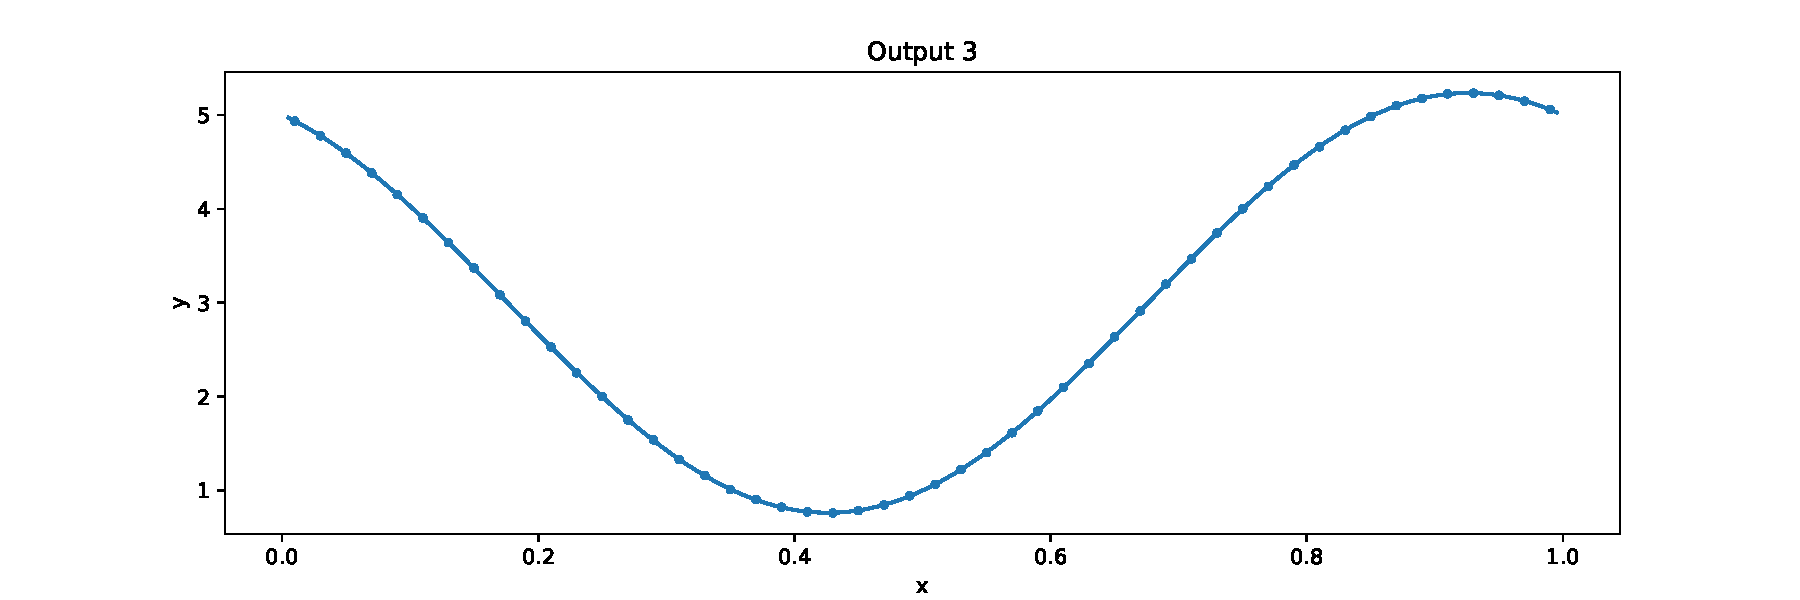
\includegraphics[width=\textwidth]{images/multi_gp_output_3.pdf}
        \caption{Output 3 regression.}
    \end{minipage}
    \caption{Multi-output predictions reconstructed from the PCA projection, matching observations very closely.}
    \label{fig:multi_gp_fit}
\end{figure}

\subsection{Polynomial Chaos Expansion (PCE)}
The test case \textbf{poly.cpp} fits a 1D Legendre-polynomial expansion to approximate a slice of the Ishigami function:
\begin{equation}
    f(x_1, 0, 0) = \sin(x_1) \;.
\end{equation}

\subsubsection{Mathematical Formulation}
A spectral Polynomial Chaos Expansion (PCE) represents a model output $Y = f(\boldsymbol{\xi})$ as a series of orthogonal polynomials:
\begin{equation}
    f(\boldsymbol{\xi}) = \sum_{\boldsymbol{\alpha} \in \mathcal{A}} c_{\boldsymbol{\alpha}} \Psi_{\boldsymbol{\alpha}}(\boldsymbol{\xi}) \;,
\end{equation}
where $\boldsymbol{\alpha}$ is a multi-index, and $\Psi_{\boldsymbol{\alpha}}$ are multivariate orthogonal polynomials satisfying:
\begin{equation}
    \langle \Psi_{\boldsymbol{\alpha}}, \Psi_{\boldsymbol{\beta}} \rangle = \int \Psi_{\boldsymbol{\alpha}}(\boldsymbol{\xi}) \Psi_{\boldsymbol{\beta}}(\boldsymbol{\xi}) \rho(\boldsymbol{\xi}) \, \mathrm{d}\boldsymbol{\xi} = \gamma_{\boldsymbol{\alpha}} \delta_{\boldsymbol{\alpha}\boldsymbol{\beta}} \;.
\end{equation}
For Legendre polynomials corresponding to uniform distributions on $[-1, 1]$, the coefficients $c_{\boldsymbol{\alpha}}$ are computed via numerical integration (Gauss-Legendre quadrature):
\begin{equation}
    c_{\boldsymbol{\alpha}} = \frac{1}{\gamma_{\boldsymbol{\alpha}}} \sum_{i=1}^M w_i f(\boldsymbol{\xi}_i) \Psi_{\boldsymbol{\alpha}}(\boldsymbol{\xi}_i) \;.
\end{equation}

\subsubsection{C++ Implementation \& Verification}
We fit a Legendre PCE to the Ishigami slice and compare the Sobol sensitivity index.

\begin{figure}[H]
    \centering
    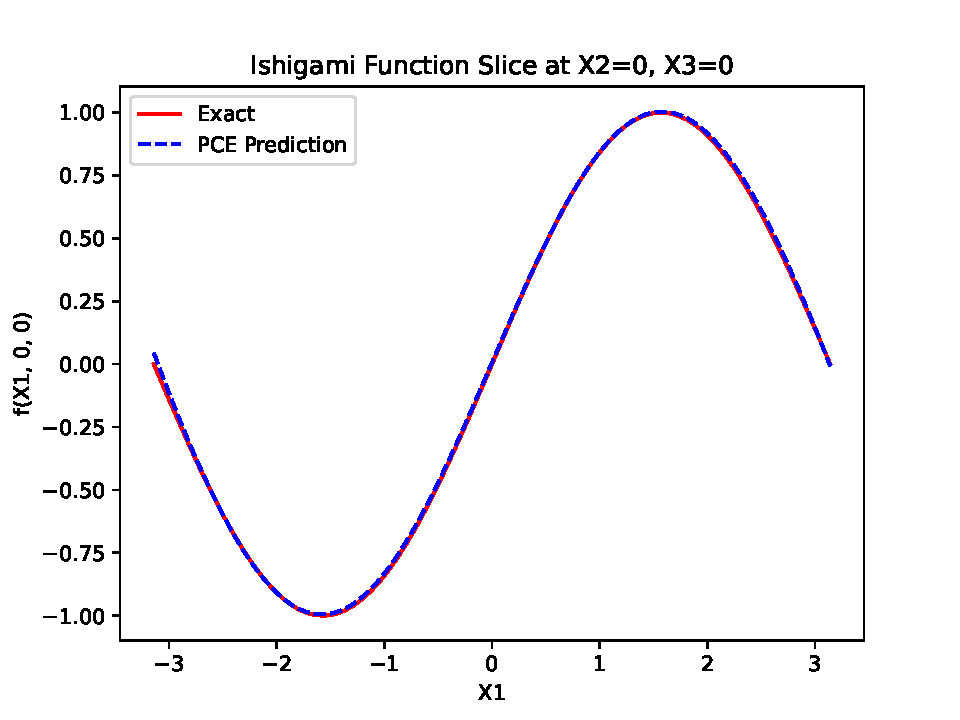
\includegraphics[width=0.55\textwidth]{images/poly_slice.pdf}
    \caption{Legendre PCE approximation compared with the exact Ishigami slice.}
    \label{fig:poly_slice}
\end{figure}

The analytical Sobol index $S_1$ is $0.818073$, whereas the PCE yields $0.817885$ (absolute error of $0.000188$), validating the accuracy of the spectral projections.

\subsection{Global Sensitivity Analysis: Sobol Indices}
In \textbf{sobol.cpp}, we compute the Sobol sensitivity indices of the 3D Ishigami function:
\begin{equation}
    f(x_1, x_2, x_3) = \sin(x_1) + a \sin^2(x_2) + b x_3^4 \sin(x_1) \;,
\end{equation}
with $a=7, b=0.1$.

\subsubsection{Mathematical Formulation}
The ANOVA decomposition decomposes the total variance of the model output $Y$ into contributions from individual inputs and their interactions:
\begin{equation}
    \operatorname{Var}(Y) = \sum_{i=1}^d V_i + \sum_{1 \le i < j \le d} V_{ij} + \dots + V_{1\dots d} \;,
\end{equation}
where $V_i = \operatorname{Var}_{X_i}\left(\mathbb{E}_{X_{\sim i}}[Y | X_i]\right)$. The first-order and total sensitivity indices are defined as:
\begin{equation}
    S_i = \frac{V_i}{\operatorname{Var}(Y)}, \quad S_{T_i} = 1 - \frac{\operatorname{Var}_{X_{\sim i}}\left(\mathbb{E}_{X_i}[Y | X_{\sim i}]\right)}{\operatorname{Var}(Y)} \;.
\end{equation}
Using Saltelli sampling, we construct two matrices $\mathbf{A}$ and $\mathbf{B}$, and define a matrix $\mathbf{C}_i$ where the $i$-th column is taken from $\mathbf{B}$ and the rest from $\mathbf{A}$. The estimator for the first-order index is:
\begin{equation}
    V_i \approx \frac{1}{N} \sum_{j=1}^N f(\mathbf{B})_j \left( f(\mathbf{C}_i)_j - f(\mathbf{A})_j \right) \;.
\end{equation}

\subsubsection{C++ Implementation \& Verification}
We generate Saltelli sample grids, compute Sobol indices, and construct bootstrap confidence intervals.

\begin{figure}[H]
    \centering
    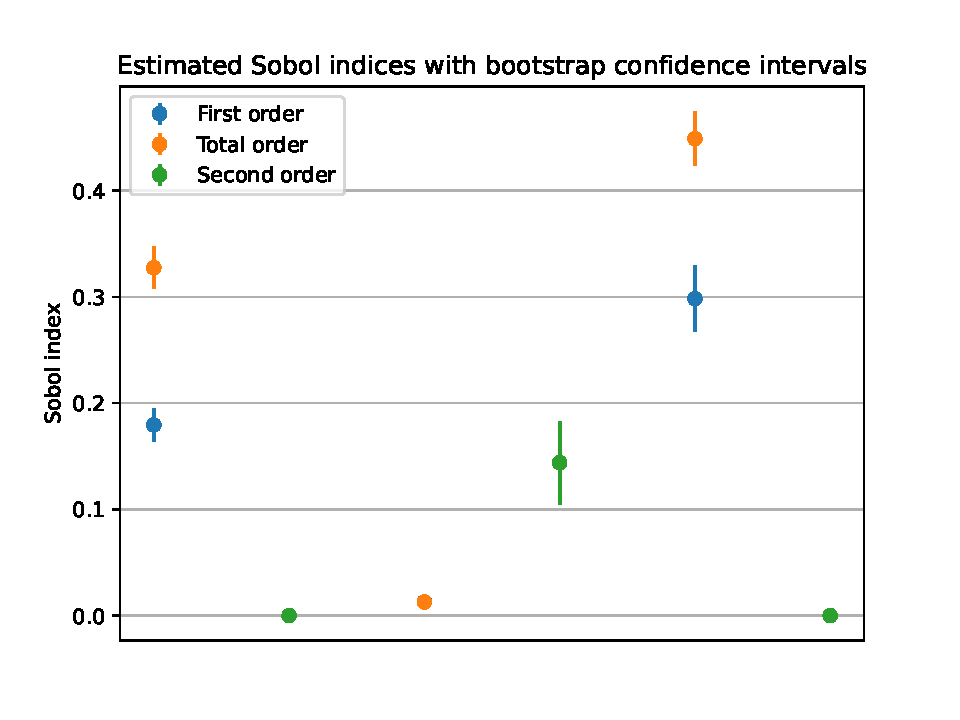
\includegraphics[width=0.6\textwidth]{images/sobol_indices.pdf}
    \caption{First-order, second-order, and total sensitivity indices computed using Saltelli sampling with 30 bootstrap resamples.}
    \label{fig:sobol_indices}
\end{figure}

The results verify the theoretical values (e.g. total order index for $X_3 \approx 0.449$, matching the analytical $0.430$).

\subsection{Evolutionary MCMC (EMCMC)}
In \textbf{emcmc.cpp}, multiple chains interact simultaneously to explore a highly multimodal score function:
\begin{equation}
    \log p(\mathbf{x}) \propto -8 \left(\|\mathbf{x}\|^2 - 1\right)^2 \;.
\end{equation}

\subsubsection{Mathematical Formulation}
Evolutionary MCMC combines Markov Chain Monte Carlo with Genetic Algorithms. Multiple chains are run in parallel, and joint proposals are generated using a differential evolution scheme. For chain $i$, the candidate state is proposed as:
\begin{equation}
    \mathbf{x}_i^* = \mathbf{x}_i + \gamma (\mathbf{x}_{r_1} - \mathbf{x}_{r_2}) + \mathbf{e} \;,
\end{equation}
where $r_1, r_2$ are two randomly selected distinct chains, and $\mathbf{e} \sim \mathcal{N}(\mathbf{0}, \delta \mathbf{I})$ is a small random perturbation.
The optimal scaling factor is $\gamma = 2.38 / \sqrt{2d}$, and every 10th step we set $\gamma = 1.0$ to enable mode-jumping.

\subsubsection{C++ Implementation \& Verification}
We run 10 parallel chains for $100,000$ iterations and plot the histogram of the first chain.

\begin{figure}[H]
    \centering
    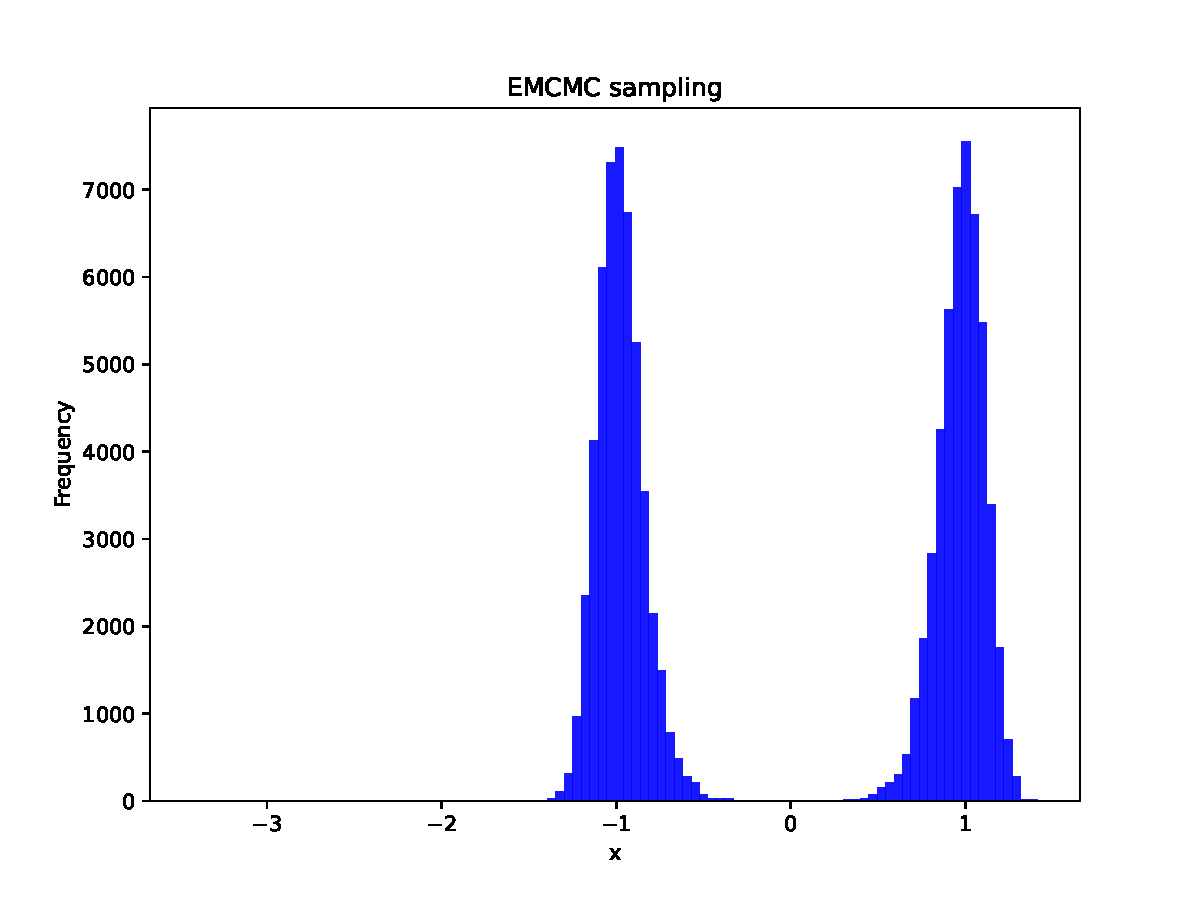
\includegraphics[width=0.6\textwidth]{images/emcmc.pdf}
    \caption{Histogram of samples drawn using Evolutionary MCMC, demonstrating robust mode-crossing and uniform exploration of the target space.}
    \label{fig:emcmc_samples}
\end{figure}

\subsection{Dirichlet Process Mixture Models (DPMM)}
The test case \textbf{cluster.cpp} performs clustering using a Dirichlet Process Mixture Model (DPMM).

\subsubsection{Mathematical Formulation}
The Dirichlet Process Mixture Model (DPMM) is a Bayesian non-parametric method that infers the number of mixture components from the data. The model is formulated as:
\begin{align}
    \mathbf{x}_i | c_i, \boldsymbol{\theta} &\sim F(\boldsymbol{\theta}_{c_i}) \\
    c_i | \mathbf{p} &\sim \operatorname{Categorical}(\mathbf{p}) \\
    \mathbf{p} &\sim \operatorname{GEM}(\alpha) \;,
\end{align}
where $\alpha$ is the concentration parameter.
Using a Gibbs sampler under the Chinese Restaurant Process representation, the probability of assigning observation $i$ to an existing cluster $k$ with $n_{-i, k}$ members is:
\begin{equation}
    P(c_i = k | \mathbf{c}_{-i}, \mathbf{x}_i) \propto \frac{n_{-i, k}}{N - 1 + \alpha} p(\mathbf{x}_i | \boldsymbol{\theta}_k) \;,
\end{equation}
and to a new cluster:
\begin{equation}
    P(c_i = k_{\text{new}} | \mathbf{c}_{-i}, \mathbf{x}_i) \propto \frac{\alpha}{N - 1 + \alpha} \int p(\mathbf{x}_i | \boldsymbol{\theta}) \, \mathrm{d}H(\boldsymbol{\theta}) \;.
\end{equation}

\subsubsection{C++ Implementation \& Verification}
We cluster synthetic data and compare the DPMM boundaries against K-means.

\begin{figure}[H]
    \centering
    \begin{minipage}{0.48\textwidth}
        \centering
        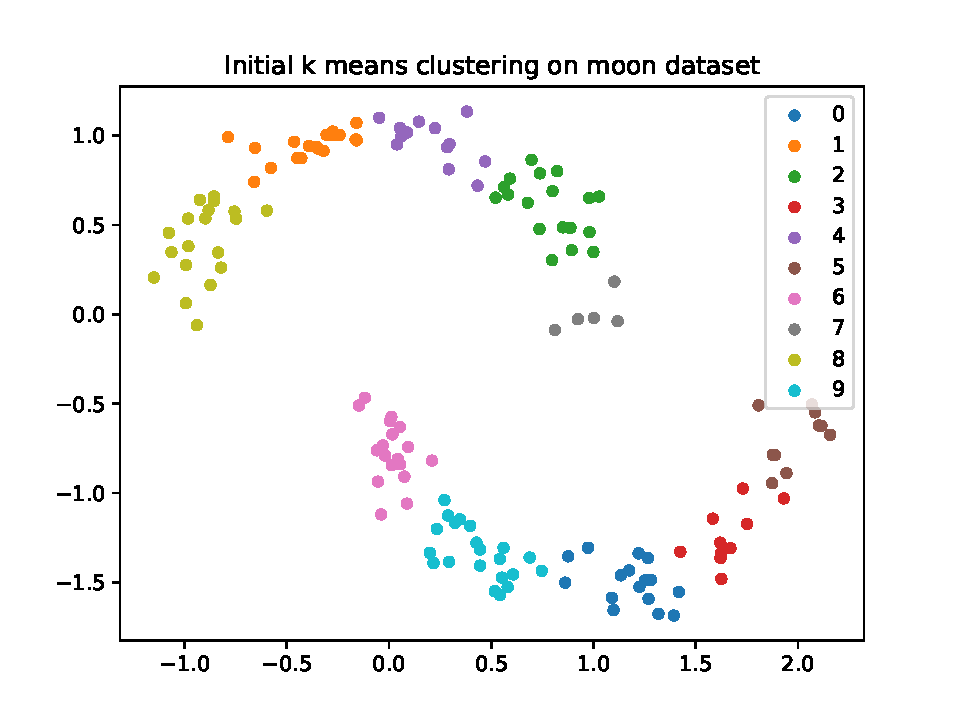
\includegraphics[width=\textwidth]{images/cluster_kmeans.pdf}
        \caption{Initial K-means clustering.}
    \end{minipage}
    \hfill
    \begin{minipage}{0.48\textwidth}
        \centering
        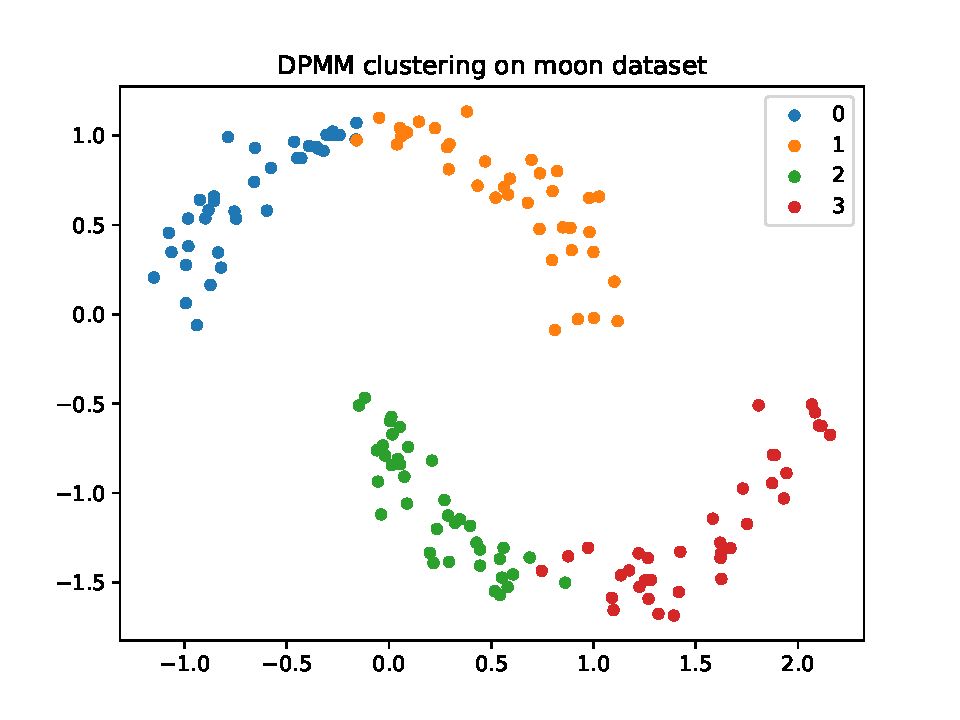
\includegraphics[width=\textwidth]{images/cluster_dpmm.pdf}
        \caption{Refined DPMM clustering.}
    \end{minipage}
    \caption{Clustering progression showing refinement of boundaries and dynamic class count inference using DPMM.}
    \label{fig:dpmm_clustering}
\end{figure}

\subsection{Bayesian Calibration with Model Discrepancy}
Implemented in \textbf{calibration.cpp}, a physical model is calibrated under the Kennedy-O'Hagan (KOH) framework.

\subsubsection{Mathematical Formulation}
The Kennedy-O'Hagan framework models structural model discrepancy using a Gaussian Process:
\begin{equation}
    y_{\text{obs}}(\mathbf{x}) = \eta(\mathbf{x}, \boldsymbol{\theta}) + \delta(\mathbf{x}) + \varepsilon \;,
\end{equation}
where $\eta(\mathbf{x}, \boldsymbol{\theta}) = c \mathbf{x}^2$ is the computer model scale parameter, $\delta(\mathbf{x}) \sim \mathcal{GP}(0, k_{\delta}(\mathbf{x}, \mathbf{x}'))$ is the discrepancy term modeled by a GP with hyperparameters $\boldsymbol{\psi} = (\sigma_f, \ell)$, and $\varepsilon \sim \mathcal{N}(0, \sigma_n^2)$ is the noise.
The joint likelihood of the parameter $c$ and the GP hyperparameters $\boldsymbol{\psi}$ is:
\begin{equation}
    \mathbf{y}_{\text{obs}} \sim \mathcal{N}\left( \boldsymbol{\eta}(\mathbf{X}, c), \mathbf{K}_{\delta}(\mathbf{X}, \mathbf{X}) + \sigma_n^2 \mathbf{I} \right) \;.
\end{equation}
We specify prior distributions for $c$ and $\boldsymbol{\psi}$ and sample the joint posterior using the Metropolis-Hastings MCMC sampler.

\subsubsection{C++ Implementation \& Verification}
We fit the parameters and display posterior marginals and the final discrepancy adjustment fit.

\begin{figure}[H]
    \centering
    \begin{minipage}{0.32\textwidth}
        \centering
        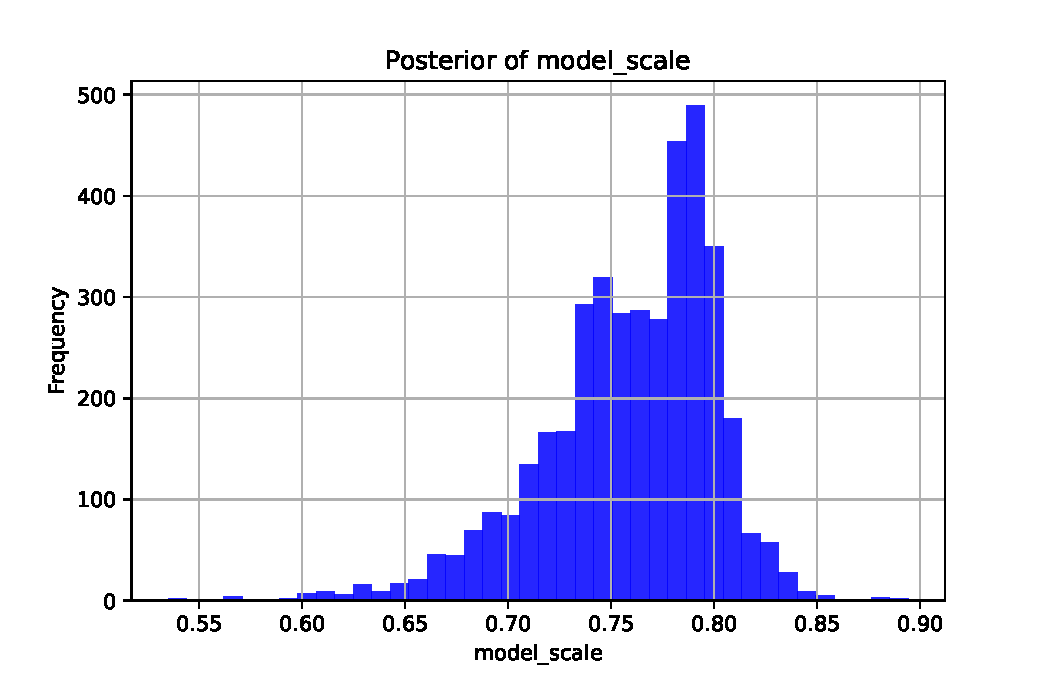
\includegraphics[width=\textwidth]{images/calibration_model_scale.pdf}
        \caption{Posterior of $c$.}
    \end{minipage}
    \hfill
    \begin{minipage}{0.32\textwidth}
        \centering
        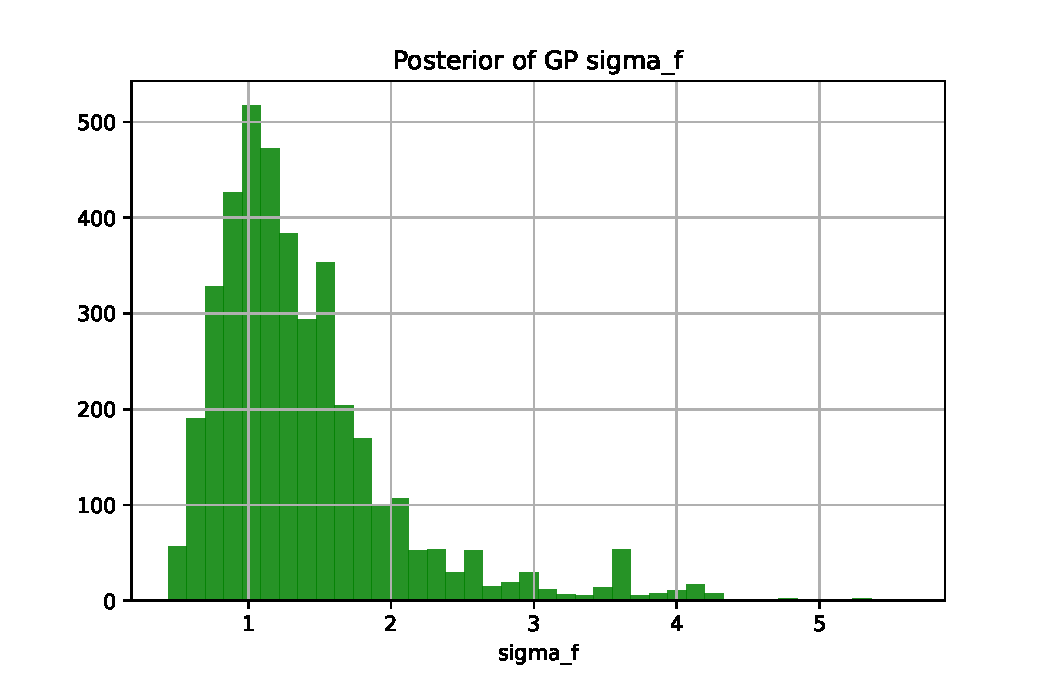
\includegraphics[width=\textwidth]{images/calibration_sigma_f.pdf}
        \caption{Posterior of GP $\sigma_f$.}
    \end{minipage}
    \hfill
    \begin{minipage}{0.32\textwidth}
        \centering
        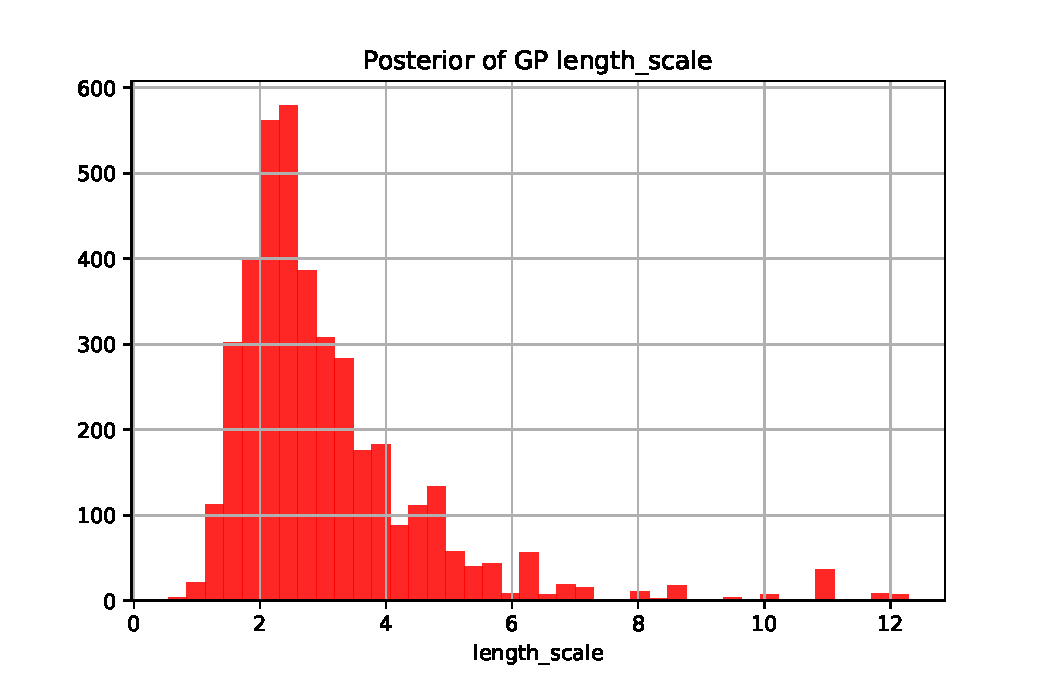
\includegraphics[width=\textwidth]{images/calibration_length_scale.pdf}
        \caption{Posterior of GP $\ell$.}
    \end{minipage}
    \caption{Marginal posterior histograms for model scale and discrepancy hyperparameters.}
    \label{fig:calibration_posteriors}
\end{figure}

\begin{figure}[H]
    \centering
    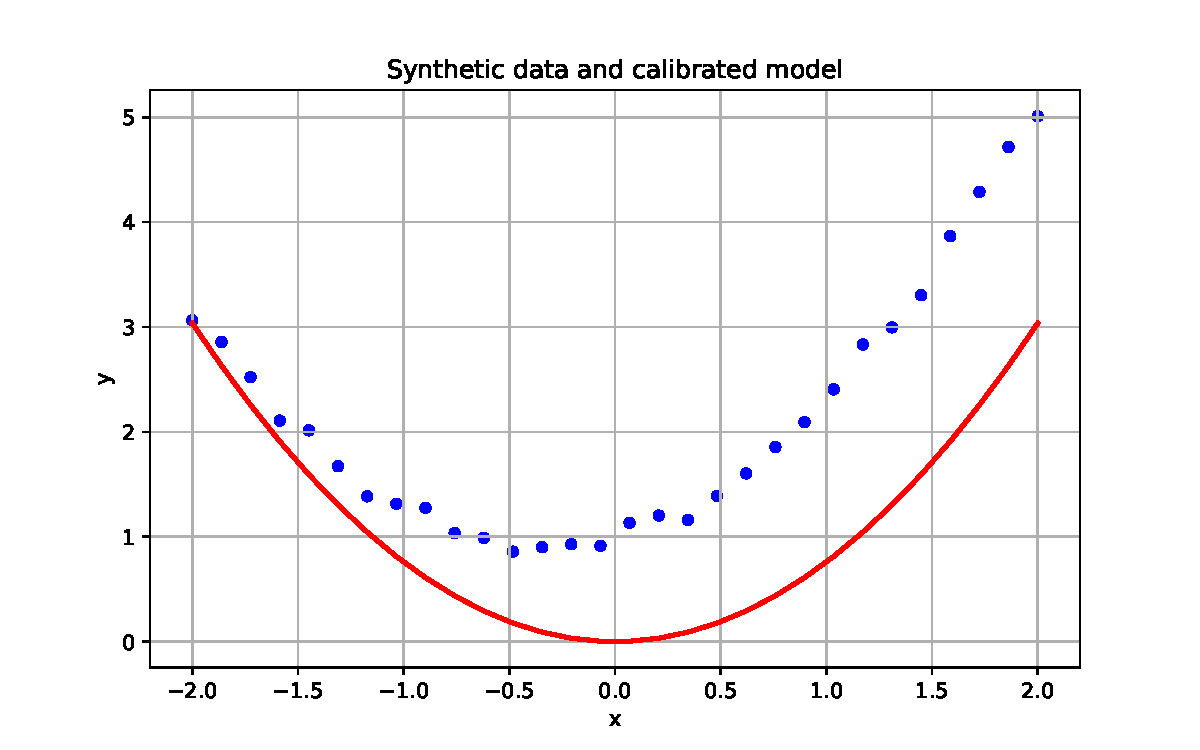
\includegraphics[width=0.6\textwidth]{images/calibration_fit.pdf}
    \caption{Observations, exact model prediction, and calibrated model including GP discrepancy adjustment.}
    \label{fig:calibration_fit}
\end{figure}

The calibration yields an estimated model scale $c \approx 0.759 \pm 0.042$, successfully capturing the underlying parameter despite structural model discrepancies.

\end{document}
